\documentclass{report}
\title{Thesis proposal: Understanding Outdoor Photometric Stereo}
\author{Yannick Hold-Geoffroy}
%\programme{Doctorat en g\'enie \'electrique}
%\annee{2015}


\date{\today}

%\usepackage{hyperref}
%\hypersetup{colorlinks,allcolors=ULlinkcolor}

%\frenchbsetup{%
%  CompactItemize=false,         % ne pas compacter les listes
%  ThinSpaceInFrenchNumbers=true % espace fine dans les nombres
%}


\usepackage[letterpaper, margin=1in]{geometry}
\usepackage[utf8]{inputenc}
\usepackage{times}
\usepackage{amsmath}
\usepackage{amssymb}
%\bibliographystyle{unsrtnat}
\usepackage[numbers,sort&compress]{natbib}
%\usepackage[numbers]{natbib}
%\usepackage{cite}   % sort citation numbers automatically
\usepackage{notoccite}
\usepackage{url}
\usepackage{graphicx}
\usepackage{rotating}
\usepackage{gensymb}
\usepackage{xcolor}
\usepackage{nicefrac}
\usepackage{placeins}
%\usepackage{adjustbox}
%\usepackage{authblk}
% to control spacing in item lists
\usepackage[titletoc]{appendix}
\usepackage{enumitem}
\usepackage[pagebackref=false,breaklinks=true,colorlinks=true,linkcolor=black,bookmarks=true]{hyperref}
\usepackage{defs}
\usepackage{amsmath,esint}
\usepackage{titlesec}
%\usepackage{breqn}
\titleformat{\chapter}[display]
  {\normalfont\sffamily\huge\bfseries}
  {}{0pt}{\Large}
\titlespacing\chapter{0pt}{12pt plus 4pt minus 2pt}{8pt plus 2pt minus 2pt}

\titleformat{\section}
  {\normalfont\sffamily\large\bfseries}
  {}{1em}{}

\titleformat{\subsection}
  {\normalfont\large\bfseries}
  {}{1em}{}

\linespread{1.5}


\begin{document}

%\frontmatter                    % pages liminaires

\maketitle
%\pagetitreonlyone                     % production des pages de titre

\tableofcontents

\hypersetup{colorlinks=true,linkcolor=blue}

% Commands
\newcommand*\B[1]{\mathbf{#1}}
\newcommand{\boldomega}{\boldsymbol \omega} % bold omega
\newcommand{\boldmu}{\boldsymbol \mu} % bold omega
\newcommand{\bolddelta}{\boldsymbol \delta} % bold delta

\newcommand\norm[1]{\left\lVert#1\right\rVert}

\newcommand\todo[1]{\textcolor{red}{TODO: #1}}

\graphicspath{{figures/}}

\chapter{Questions by Denis Laudenreau}

\section{Question 1}

\subsection{(a)}
\textbf{What is the illuminance $E_{\text{strip}}$ at point $P$ lying on a plane parallel to the $yz$ plane and located opposite the middle of the strip and at a distance $r$?}

Suppose q as the distance between the strip light and P along the x-axis.

\begin{figure}
  \centering
  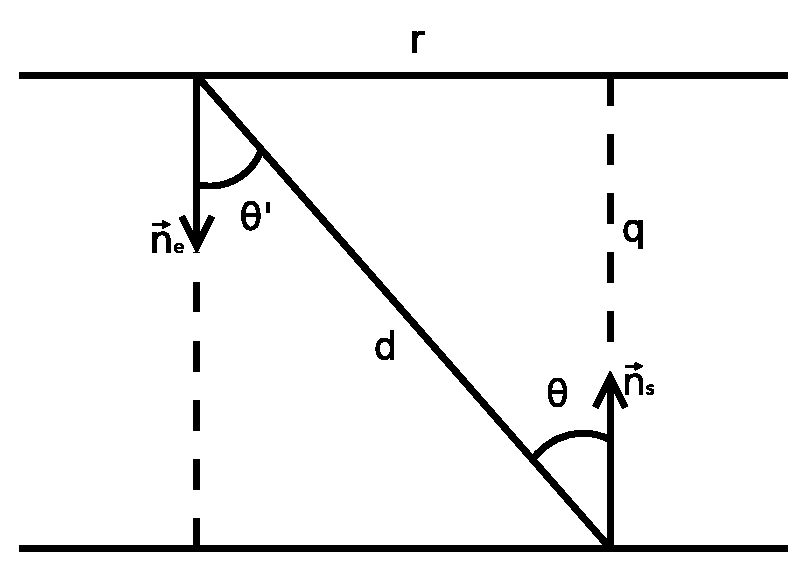
\includegraphics[width=0.45\linewidth]{q1a_setup.eps}
  \caption[Problem setup]
   {Top-down view of the problem. Note that $\theta = \theta'$.}
  \label{q1a:setup}
\end{figure}

The irradiance equation is defined as \todo{1/pi???}
\begin{equation}
E(r) = \frac{1}{\pi} \int_{\Omega} L(r,\omega)\cos(\theta) d\omega
\quad,
\end{equation}
where $L(r,\omega)$ is the radiance of the emitting surface and $\theta$ is the angle between the receiving surface normal and the light ray, for the whole hemisphere lighting the surface $\Omega$.

In Cartesian coordinates, this can be written as
\begin{equation}
E(r) = \int\limits_{z= -r - \frac{W}{2}}^{-r+\frac{W}{2}} \int\limits_{y= - \frac{H}{2}}^{\frac{H}{2}} L \cos(\theta) d\omega
\quad,
\label{q1a:irr}
\end{equation}
as $L$ is constant over the surface.

It is possible to rewrite $\cos(\theta)$ as
\begin{align}
\cos(\theta)  &= \frac{q}{d} \\
              &= \frac{q}{\sqrt{q^2 + y^2 + z^2}}
\quad,
\label{q1a:cos}
\end{align}
and $d\omega$ as
\begin{align}
d\omega &= \frac{\cos(\theta)}{d^2} dA \\
        &= \frac{q}{d} \frac{1}{d^2} dA \\
        &= \frac{q}{\left(q^2 + y^2 + z^2\right)^\frac{3}{2}} dA
\quad.
\label{q1a:dw}
\end{align}

Rewriting equation equation \eqref{q1a:irr} using equations \eqref{q1a:cos} and \eqref{q1a:dw} gives
\begin{align}
E(r) &= \int\limits_{z= -r - \frac{W}{2}}^{-r+\frac{W}{2}} \int\limits_{y= - \frac{H}{2}}^{\frac{H}{2}} L \frac{q}{\sqrt{q^2 + y^2 + z^2}} \frac{q}{\left(q^2 + y^2 + z^2\right)^\frac{3}{2}} dydz \\
     &= L \int\limits_{z= -r - \frac{W}{2}}^{-r+\frac{W}{2}} \int\limits_{y= - \frac{H}{2}}^{\frac{H}{2}} \frac{q^2}{\left(q^2 + y^2 + z^2\right)^2} dydz 
     %&= L \int\limits_{z= -r - \frac{W}{2}}^{-r+\frac{W}{2}} - \frac{q^2\, \arctan\!\left(\frac{y}{\sqrt{q^2 + z^2}}\right)}{2\, {\left(q^2 + z^2\right)}^{\frac{3}{2}}} - \frac{q^2\, y}{2\, \left(q^2 + z^2\right)\, \left(q^2 + y^2 + z^2\right)} \Big|_{-\frac{H}{2}}^{\frac{H}{2}} dz \\
     %&= L \int\limits_{z= -r - \frac{W}{2}}^{-r+\frac{W}{2}} - \frac{q^2\, \arctan\!\left(\frac{H}{2\, \sqrt{q^2 + z^2}}\right)}{{\left(q^2 + z^2\right)}^{\frac{3}{2}}} - \frac{H\, q^2}{2\, \left(q^2 + z^2\right)\, \left(\frac{H^2}{4} + q^2 + z^2\right)} dz \\
\quad.
\end{align}

\subsection{(b)}
\textbf{ What becomes the expression of $E_{\text{strip}}$ found in (a) when the length H of the light strip is very large with respect to the distance r between the center point of the strip and $P$ ?}

As H gets bigger, making the fraction $\frac{-h^2}{\left(h^2 + y^2 + z^2\right)^2}$ tend towards $0$ for, as the values of $y$ grows bigger while the rest stay constant.

The way the irradiance $E(r)$ is defined in cartesian coordinates in (a) won't give us insights on this question. As such, it is more interesting to derive the same irradiance $E(r)$ in spherical coordinates:
\begin{align}
E(r) &= \frac{1}{\pi} \int\limits_{-\arctan(\frac{\frac{H}{2}}{\sqrt{q^2+r^2}})}^{\arctan(\frac{\frac{H}{2}}{\sqrt{q^2+r^2}})} \int\limits_{\arctan \left(\frac{r-\frac{W}{2}}{q} \right)}^{\arctan \left(\frac{r+\frac{W}{2}}{q} \right)} L \cos(\theta) \sin(\theta) d\theta d\phi \\
     &= 2 L \cdot \arctan \left(\frac{\frac{H}{2}}{\sqrt{q^2+r^2}}\right) \cdot \int\limits_{\arctan \left(\frac{r-\frac{W}{2}}{q} \right)}^{\arctan \left(\frac{r+\frac{W}{2}}{q} \right)} \cos(\theta) \sin(\theta) d\theta \\
     &= 2 L \cdot \arctan \left(\frac{H}{2\sqrt{q^2+r^2}} \right) \cdot \left[ - \frac{1}{2} \cos^2(x) \right]_{\arctan(\frac{r-W/2}{q})}^{\arctan \left(\frac{r+W/2}{q} \right)} \\
     &= 2 L \cdot \arctan \left(\frac{H}{2\sqrt{q^2+r^2}} \right) \cdot \left[ - \frac{1}{2} \cos^2\left(\arctan\left(\frac{r+W/2}{q}\right)\right) - - \frac{1}{2} \cos^2\left(\arctan\left(\frac{r-W/2}{q}\right)\right) \right] \\
     &= 2 L \cdot \arctan\!\left(\frac{H}{2\, \sqrt{q^2 + r^2}}\right) \cdot \left(\frac{1}{2\, \left(\frac{{\left(\frac{W}{2} - r\right)}^2}{q^2} + 1\right)} - \frac{1}{2\, \left(\frac{{\left(\frac{W}{2} + r\right)}^2}{q^2} + 1\right)}\right)
     \label{q1b:irr_sph}
\end{align}

As can be seen from eq.~\eqref{q1b:irr_sph}, having a large $H$ in the $\arctan$ makes the left part of the equation equal to $2 \cdot \frac{\pi}{2}$:
\begin{equation}
E(r) = \pi L \left(\frac{1}{2\, \left(\frac{{\left(\frac{W}{2} - r\right)}^2}{q^2} + 1\right)} - \frac{1}{2\, \left(\frac{{\left(\frac{W}{2} + r\right)}^2}{q^2} + 1\right)}\right)
\end{equation}

\subsection{(c)}
\textbf{What is the expression of the illuminance $E_{\text{tube}}$ at $P$ as a function of $E_{\text{strip}}$ ?
What is the expression of this illuminance $E_{\text{tube}}$ when $r$ is equal to 0?}

Supposing $r$ stays roughly the same, the difference is that the $\cos(\theta)$ factor should be removed, as there is always a complete cylinder cross-section shining on the surface element (?) P, as can be seen in fig.~\ref{q1c:setup}. This means that the expression of $E_{\text{tube}}$ is
\begin{align}
E_{\text{tube}} &= E_{\text{strip}} \frac{1}{\cos(\theta)} \\
                &= E_{\text{strip}} \frac{\sqrt{q^2+y^2+z^2}}{q}
\quad.
\end{align}

\begin{figure}
  \centering
  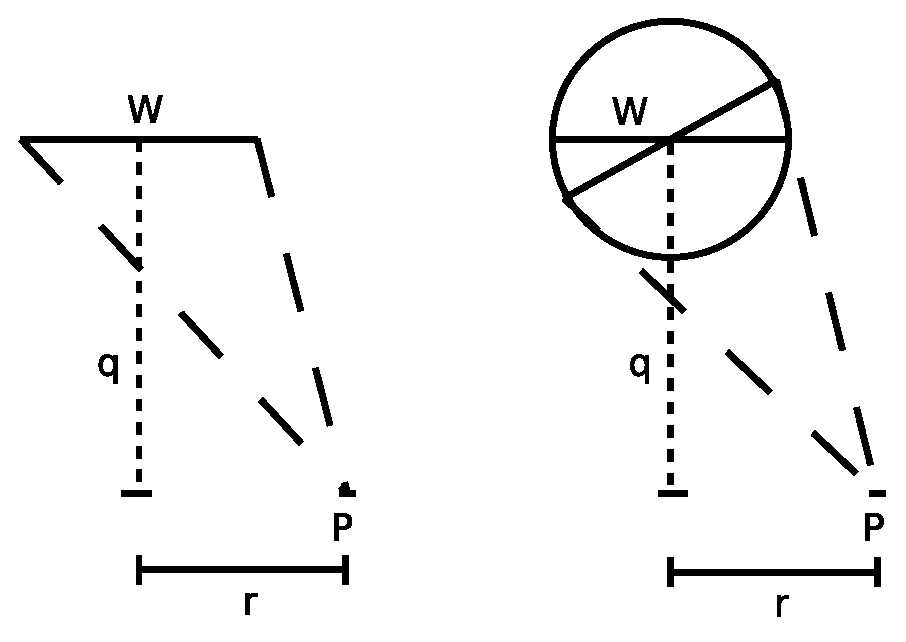
\includegraphics[width=0.45\linewidth]{q1c_setup.eps}
  \caption[Problem setup]
   {Top-down view of the strip and a tube lighting P.}
  \label{q1c:setup}
\end{figure}

\section{Question 2}
\subsection{(a)}
\textbf{What is the expression of the illuminance at $P$ ?}

Let's start with the irradiance integral,
\begin{equation}
E(r) = \frac{1}{\pi} \int_{\Omega} L(r,\omega)\cos(\theta) d\omega
\quad.
\end{equation}
As the luminance is constant, $L(r,\omega)$ can be changed to $L$. When solving 

\begin{align}
E(r) &= \int_{0}^{\arctan(\frac{h}{q})} \int_{0}^{\arctan(\frac{w}{q})} L\cos(\theta) \sin(\theta) d\theta d\phi \\
     &= \arctan\left(\frac{h}{q}\right) \cdot \int_{0}^{\arctan(\frac{w}{q})} L\cos(\theta) \sin(\theta) d\theta \\
     %&= \arctan(\frac{h}{q}) \cdot \left[ - \frac{1}{2} \cos^2(x) \right]_{0}^{\arctan(\frac{w}{q})} \\
     %&= \arctan(\frac{h}{q}) \cdot \left[ - \frac{1}{2} \cdot \cos^2(\arctan(\frac{w}{q})) - -\frac{1}{2} \right] \\
     %&= - \arctan\!\left(\frac{h}{q}\right)\, \left(\frac{1}{2\, \sqrt{\frac{w^2}{q^2} + 1}} - \frac{1}{2}\right)
     &= \arctan\left(\frac{h}{q}\right) \cdot \frac{w^2}{2 \left(q^2 + w^2\right)} L
\end{align}


%\begin{equation}
%E(r) = \frac{L}{2\pi} \sum_{i=1}^{n} \beta_i \cos(\alpha_i)
%\end{equation}
%\begin{align*}
%E(r) &= \frac{L}{2\pi} \left( \arctan(\frac{w}{q}) + \arctan(\frac{h}{q}) + \arctan(\frac{w}{q}) \cdot \cos(\arctan(\frac{h}{q})) + \arctan(\frac{w}{q}) \cdot \cos(\arctan(\frac{w}{q})) \right) \\
%     &= \arctan\!\left(\frac{w}{q}\right) + \arctan\!\left(\frac{h}{q}\right) + \frac{\arctan\!\left(\frac{w}{q}\right)}{\sqrt{\frac{h^2}{q^2} + 1}} + \frac{\arctan\!\left(\frac{h}{q}\right)}{\sqrt{\frac{w^2}{q^2} + 1}}
%\end{align*}

\subsection{(b)}
\textbf{What is the illuminance at $P$ if the light plane is the one shown in~\ref{q2b:setup}?}

\begin{figure}
  \centering
  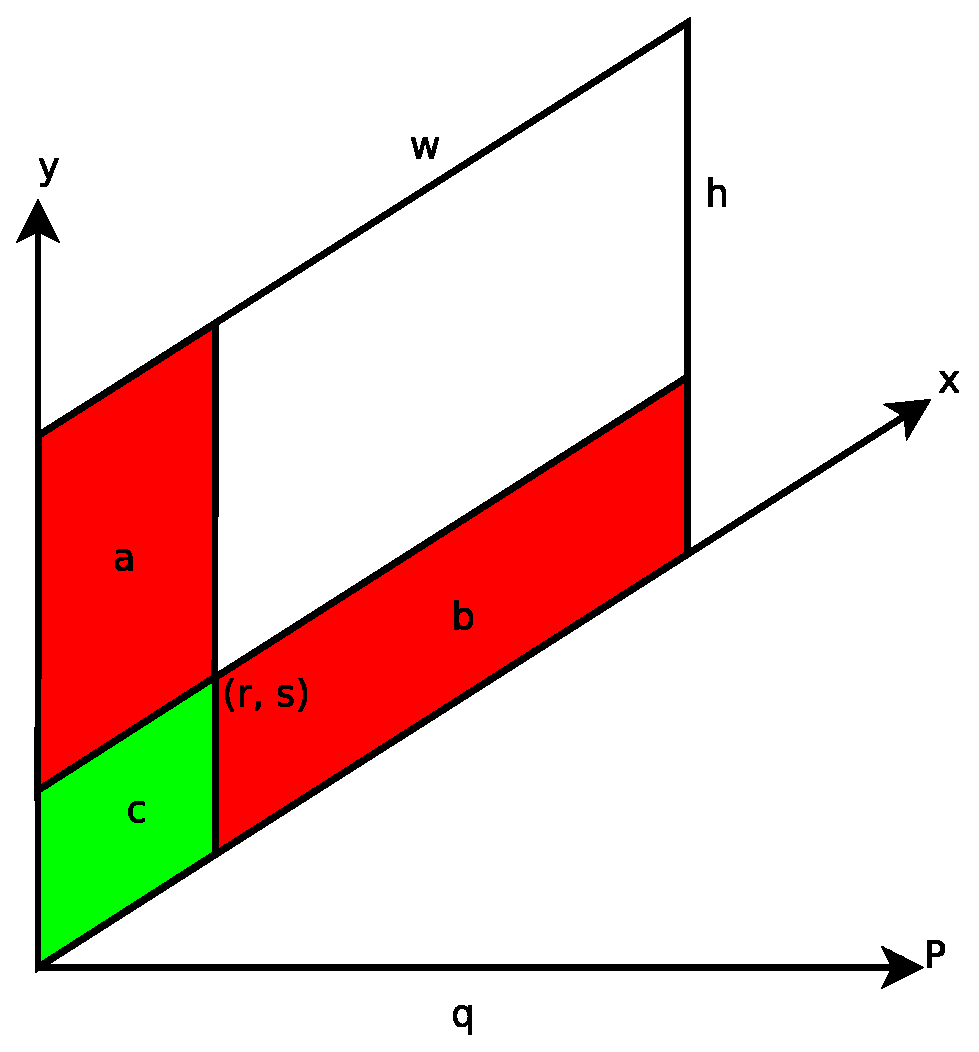
\includegraphics[width=0.2\linewidth]{q2b_setup.eps}
  \caption[Problem setup]
   {Problem setup.}
  \label{q2b:setup}
\end{figure}

The setup of this surface makes shifts the lower bounds of the definite integral from $0$ to some arbitrary value $r$ and $s$ on the $x$ and $y$ axis, respectively. Instead of performing the integral again, it is possible to use a simple trick, as shown in fig~\ref{q2b:setup}. The new surface $w \times h$ can be derived from the previous answer (for a surface $r+w \times s+h$). All is left to do is subtract the extraneous surfaces $a$, $b$ and $c$. To do so, it is possible to reuse the previous answer to find surface $a+c$ and $b+c$, and then re-add $c$, as it was subtracted twice (the inclusion-exclusion principle). The answer is then
\begin{align*}
E(r) =& \biggl( \arctan\left(\frac{s+h}{q}\right) \cdot \frac{\left(r+w\right)^2}{2 \left(q^2 + \left(r+w\right)^2\right)}
- \arctan\left(\frac{s+h}{q}\right) \cdot \frac{\left(r\right)^2}{2 \left(q^2 + r^2\right)} \\
&- \arctan\left(\frac{s}{q}\right) \cdot \frac{\left(r+w\right)^2}{2 \left(q^2 + \left(r+w\right)^2\right)}
+ \arctan\left(\frac{s}{q}\right) \cdot \frac{\left(r\right)^2}{2 \left(q^2 + r^2\right)} \biggr) L
\quad.
\end{align*}

\chapter{Questions by Philippe Giguère}

\section{Question 3}

\textbf{Impact of estimated light source error vs. estimated normal error (bias).}

The setup for this experiment is shown in fig.~\ref{q3:setup}. Three light sources forms an triangular pyramid with an equilateral triangle as its base. The problem states that its edge central angle is $r$.

\begin{figure}
  \centering
  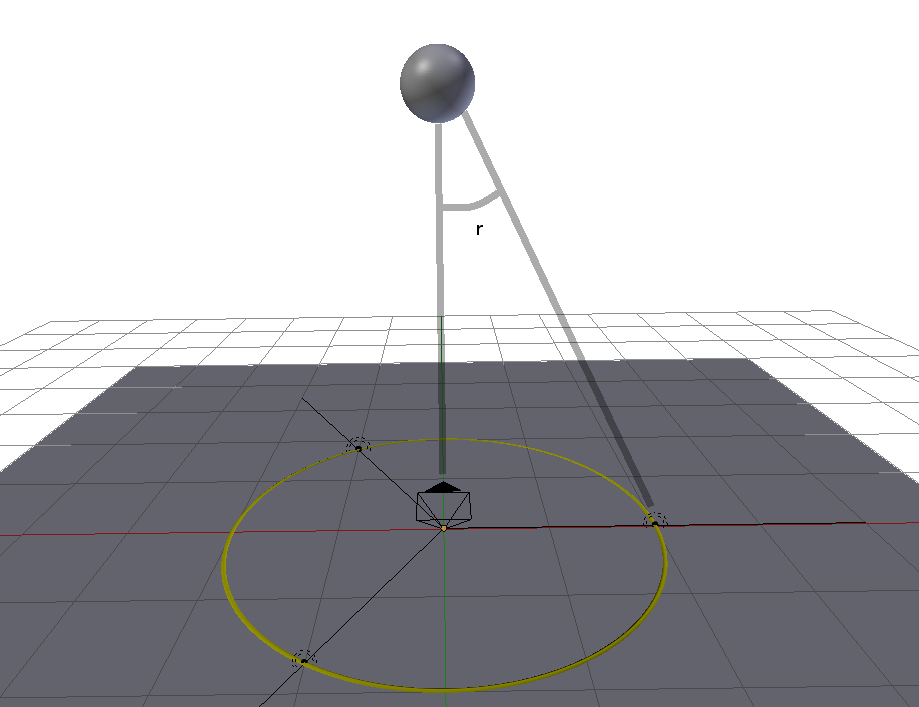
\includegraphics[width=0.9\linewidth]{q3_setup.png}
  \caption[Experiment setup]
   {Experiment setup.}
  \label{q3:setup}
\end{figure}

On this setup, each light, when lit, generate a row $\B{l}$ in the lighting matrix $\B{L}$ as such:
\begin{equation}
\B{l} =
\left[\begin{array}{c} \cos\!\left(\theta\right)\, \sin\!\left(r\right) \\ \sin\!\left(r\right)\, \sin\!\left(\theta\right) \\ \sqrt{ - {\cos\!\left(\theta\right)}^2\, {\sin\!\left(r\right)}^2 - {\sin\!\left(r\right)}^2\, {\sin\!\left(\theta\right)}^2 + 1} \end{array}\right]^T
\quad .
\end{equation}
The $x$ and $y$ components are directly the position on the plane, while the $z$ component is specified to make the light unit, so they are all the same intensity.

In the current setup, since the lights are on the vertex of an equilateral triangle, they are $120\degree$ apart on the $xy$-plane, so $\theta = \left[ 0\degree, 120\degree, 240\degree \right]$. This translates in the following lighting matrix:
\begin{equation}
\B{L} =
\left[\begin{array}{ccc} \sin\!\left(r\right) & 0 & \sqrt{1 - {\sin\!\left(r\right)}^2}\\ -\frac{\sin\!\left(r\right)}{2} & \frac{\sqrt{3}\, \sin\!\left(r\right)}{2} & \sqrt{1 - {\sin\!\left(r\right)}^2}\\ -\frac{\sin\!\left(r\right)}{2} & -\frac{\sqrt{3}\, \sin\!\left(r\right)}{2} & \sqrt{1 - {\sin\!\left(r\right)}^2} \end{array}\right]
\quad .
\end{equation}

Given the simple lambertian reflectance equation (supposing unit albedo), we can compute the pixel intensity of a camera pointed directly to a surface with normal $\B{n}$:
\begin{equation}
b = \B{L}\B{n}
\quad.
\end{equation}
Photometric Stereo is the inverse process, where the normals $\B{n} = \left[ n_x \; n_y \; n_z\right]^T$ are solved from the lighting matrix $\B{L}$ and the pixel intensity $b$. This can be done by inverting the light matrix $\B{L}$, as such:
\begin{equation}
\B{L}^{-1}\B{b} = \B{n} = 
\begin{bmatrix}
n_x \\
n_y \\
n_z 
\end{bmatrix}
\quad.
\end{equation}
We can see that, unless matrix $\B{L}$ is singular or affected by noise, we retrieve the three components of the normal $\B{n}$ directly.

But, instead of solving the usual equation, the problem suppose we have a systematic error $\epsilon_r$ in the measurement of $r$, making the noisy lighting matrix $\B{L}_\epsilon$ a bit different that the original matrix:
\begin{equation}
\B{L}_\epsilon = \left[\begin{array}{ccc} \sin\!\left(\epsilon_r + r\right) & 0 & \sqrt{1 - {\sin\!\left(\epsilon_r + r\right)}^2}\\ -\frac{\sin\!\left(\epsilon_r + r\right)}{2} & \frac{\sqrt{3}\, \sin\!\left(\epsilon_r + r\right)}{2} & \sqrt{1 - {\sin\!\left(\epsilon_r + r\right)}^2}\\ -\frac{\sin\!\left(\epsilon_r + r\right)}{2} & -\frac{\sqrt{3}\, \sin\!\left(\epsilon_r + r\right)}{2} & \sqrt{1 - {\sin\!\left(\epsilon_r + r\right)}^2} \end{array}\right]
\quad.
\end{equation}
Solving this problem gives us:
\begin{equation}
\B{L}_\epsilon^{-1}\B{b} = \B{n}_\epsilon = 
\left[\begin{array}{c} n_x \cdot \frac{\sin\!\left(r\right)}{\sin\!\left(\epsilon_r + r\right)}\\ n_y \cdot \frac{\sin\!\left(r\right)}{\sin\!\left(\epsilon_r + r\right)}\\ n_z \cdot \frac{\sqrt{1 - {\sin\!\left(r\right)}^2}}{\sqrt{1 - {\sin\!\left(\epsilon_r + r\right)}^2}} \end{array}\right] =
\begin{bmatrix}
n_x \cdot \Delta_{\epsilon_x} \\
n_y \cdot \Delta_{\epsilon_y} \\
n_z \cdot \Delta_{\epsilon_z} \\
\end{bmatrix}
\quad,
\end{equation}
where the normal components $n_x$, $n_y$ and $n_z$ are all multiplied by a non-unit factor due to the measurement error $\epsilon_r$. Note that $\Delta_{\epsilon_x} = \Delta_{\epsilon_y}$. These factors are shown in fig.~\ref{q3:analytical}. Given a large measure error ($\epsilon_r$ near $30\degree$ or $-30\degree$), it is interesting to note that the $x$ and $y$-axis components of the recovered normal are more stable given a large lighting triangle (high value of $r$), while the $z$-axis component is more stable at lower values of $r$. Globally, the $x$ and $y$-axis components are more unstable, as even with no measurement error ($\epsilon_r = 0\degree$), they cannot be solved accurately for small values of $r$.

\begin{figure}
  \centering
  \begin{tabular}{cc}
  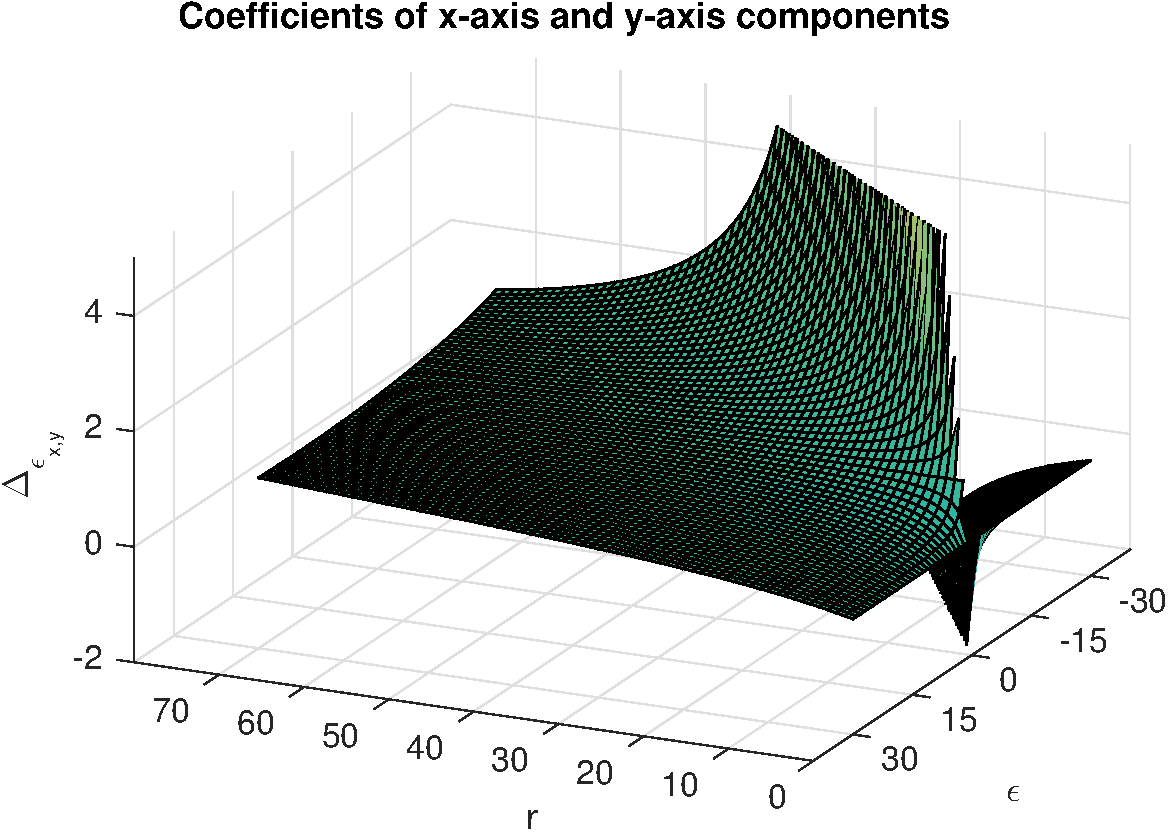
\includegraphics[width=0.45\linewidth]{q3_analytic_nx_ny.pdf} &
  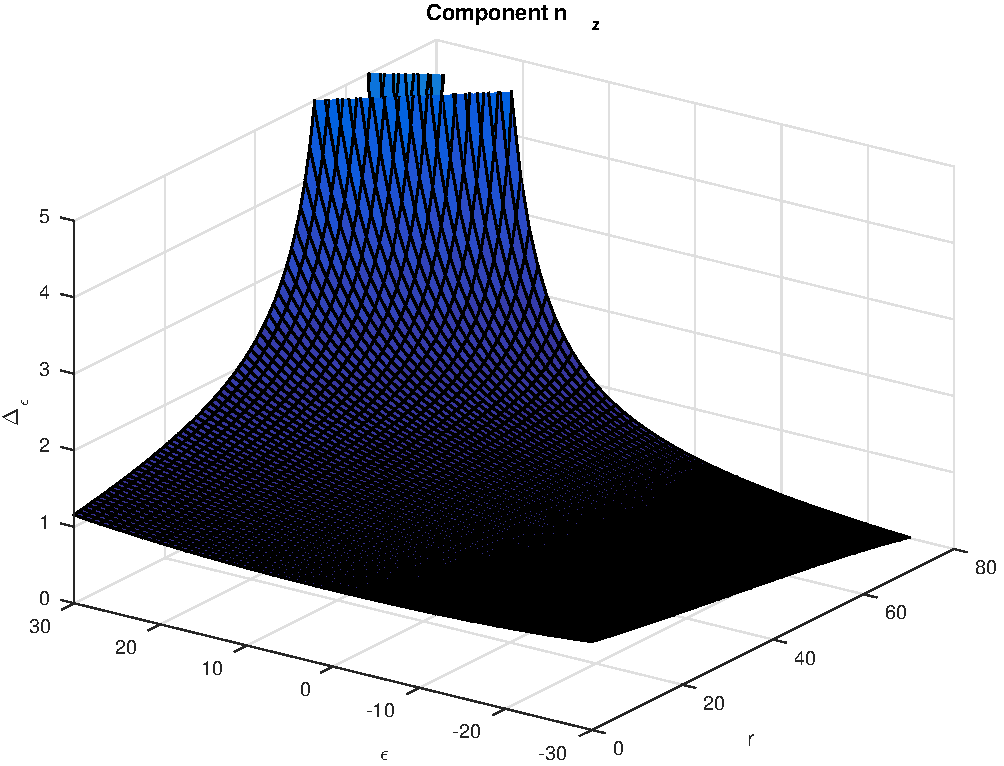
\includegraphics[width=0.45\linewidth]{q3_analytic_nz.pdf} \\
  (a) & (b)
  \end{tabular}
  \caption[Analytical normal component coefficients]
   {The theoretical factor $\Delta_\epsilon$ that multiplies each normal component (a) $n_x$, $n_y$ and (b) $n_z$ in the presence of a measure error $\epsilon_r$. When the factor is 1, no error is made on this component during the reconstruction (as it is the case when $\epsilon = 0$). A value less than 1 means the reconstructed normal component is smaller than the ground truth, while a value over 1 means a bigger component than the ground truth.}
  \label{q3:analytical}
\end{figure}

Until now, the noise impact was given analytically. If we try to actually perform a reconstruction on simulated data, there is something important to take into account that was left behind in the analytical analysis, namely the noise. The conditioning of the matrix $\B{L}$ is an interesting stability measure, as it bounds the stability of the solution when noise disturbs the matrix. This is even more related to this particular question because of the definition of the conditioning of the matrix $\kappa \left(\B{L}\right)$, as related by~\cite{ElGhaoui2002},
\begin{equation}
\frac{ \| \B{L}_\epsilon ^{-1} - \B{L}^{-1} \| }{ \| \B{L}^{-1} \| }
\le \kappa\left(\B{L} \right) \frac{ \| \B{L}_\epsilon - \B{L}  \| }{ \| \B{L} \| }
\quad,
\end{equation}
where $\kappa \left(\B{L}\right) = \|\B{L}\| \cdot \|\B{L}^{-1}\|$. As~\cite{ElGhaoui2002} explains, ``the classical condition number $\kappa \left(\B{L}\right)$ is a measure of (relative) errors in the inverse of A when the latter is perturbed by an arbitrary, infinitesimally small matrix.''.

Two experiments are presented: first, a surface normal $\B{n}$ is fixed while the lighting angle $r$ and measurement error $\epsilon_r$ varies. The results are presented in fig.~\ref{q3:exp1}. In the second experiment, a given lighting angle $r$ is fixed, while the surface normal $\B{n}$ and the measurement error $\epsilon_r$ varies. The results are shown in fig~\ref{q3:exp2} and \ref{q3:exp2a}. In both experiments, the angular error and reciprocal condition number $\nicefrac{1}{\kappa\left(L\right)}$ are displayed.

\begin{figure}
  \centering
  \begin{tabular}{ccc}
  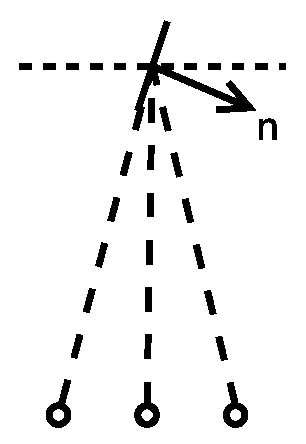
\includegraphics[width=0.2\linewidth]{q3_surface_normal_18-5.eps} &
  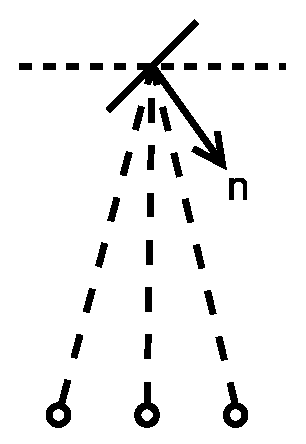
\includegraphics[width=0.2\linewidth]{q3_surface_normal_45.eps} &
  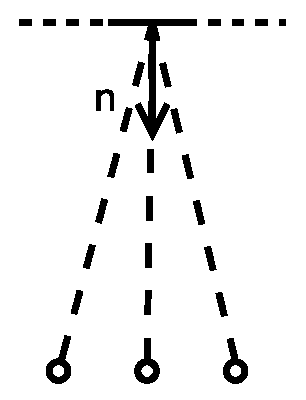
\includegraphics[width=0.2\linewidth]{q3_surface_normal_90.eps} \\
  (a) & (b) & (c)
  \end{tabular}
  \caption[Surface normal examples]
   {Top-down view of three example surfaces normals where $\theta_{\text{azimuth}}$ is (a) $18.5\degree$, (b) $45\degree$ and (c) $90\degree$.}
  \label{q3:angle_setup}
\end{figure}

\begin{figure}
  \centering
  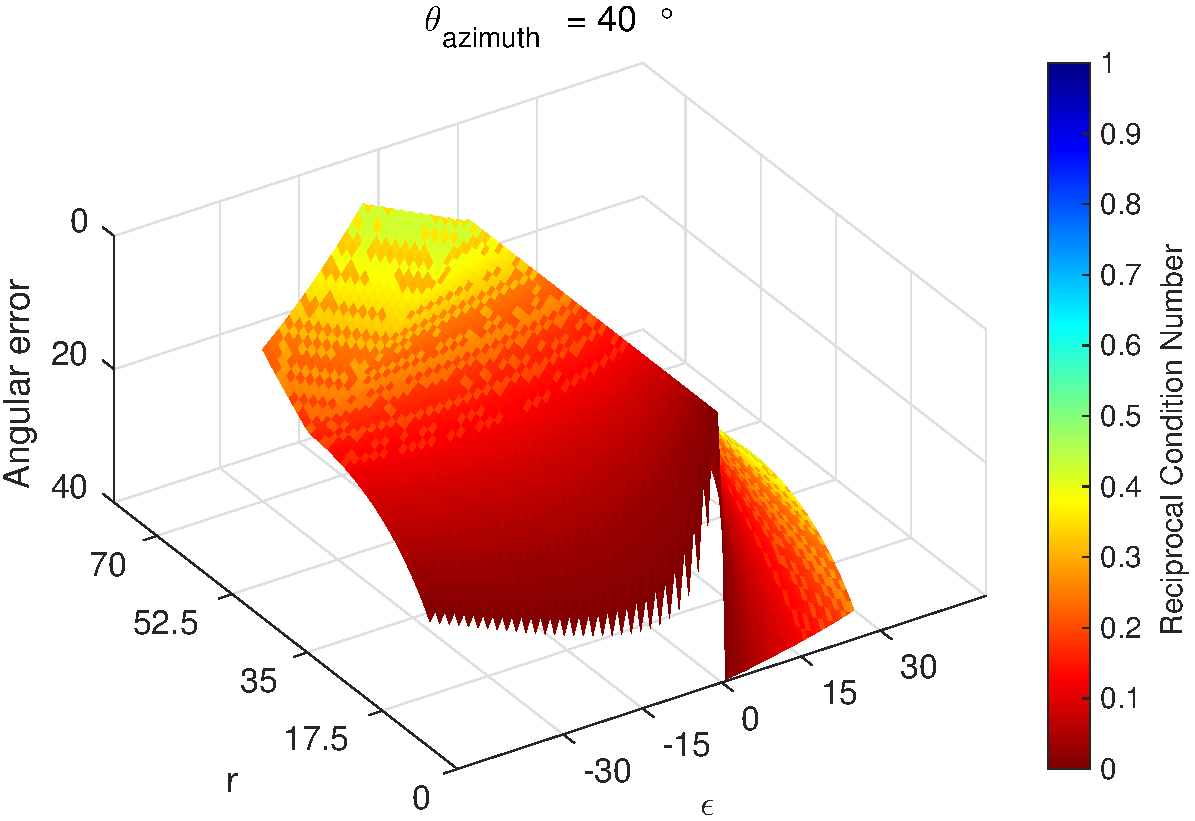
\includegraphics[width=0.45\linewidth]{q3_experiment_1_view_1.pdf}
  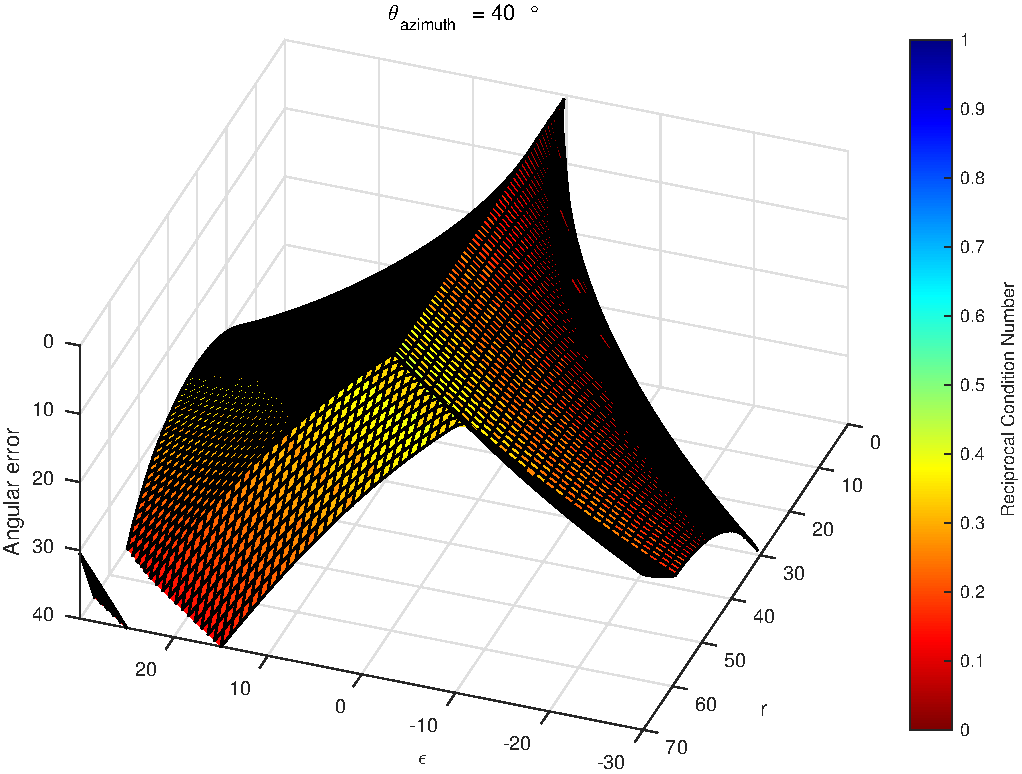
\includegraphics[width=0.45\linewidth]{q3_experiment_1_view_2.pdf}
  \caption[Experiment 1]
   {Angular error in degrees (z-axis) and reciprocal condition number (color) in function of $r \in \left[0, 70\right]$ (y-axis) and $\epsilon_r \in \left[-30, 30\right]$ (x-axis). The surface ground truth $\theta_{\text{azimuth}}$ is set to 40\degree on the plane containing the first light, the center of the triangle and the surface element to reconstruct (see fig.~\ref{q3:angle_setup}). Both figures are two different point of views of the same function. Note how the region around $r = 30$ and $\epsilon = 10$ have a relatively good conditioning, but the result is much worse than regions with a lower measurement error $\epsilon$.}
  \label{q3:exp1}
\end{figure}



\begin{figure}
  \centering
  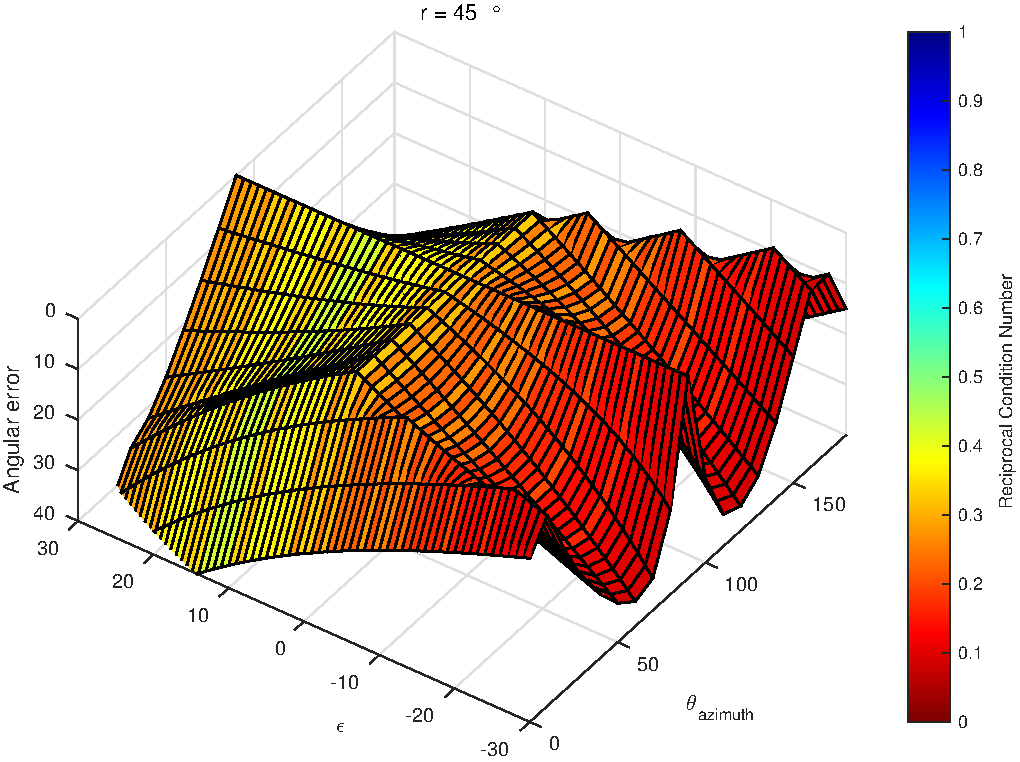
\includegraphics[width=0.45\linewidth]{q3_experiment_2_view_1.pdf}
  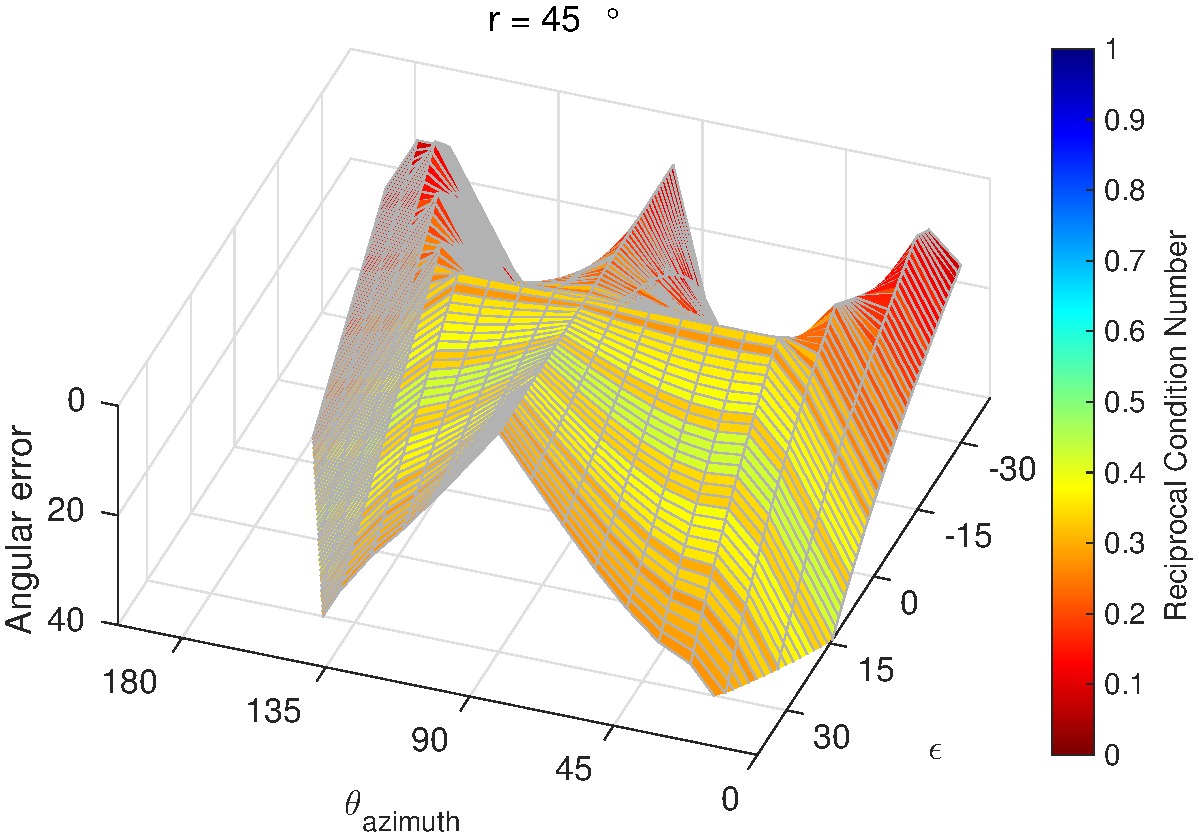
\includegraphics[width=0.45\linewidth]{q3_experiment_2_view_2.pdf}
  \caption[Experiment 2]
   {Angular error in degrees (z-axis) and reciprocal condition number (color) in function of $\theta_{\text{azimuth}} \in \left[0, 180\right]$ (y-axis) and $r \in \left[0, 70\right]$ (x-axis). Some example angles for $\theta_{\text{azimuth}}$ are shown in fig.~\ref{q3:angle_setup}. Both figures are two different point of views of the same function. Note how the region around $r = 30$ and $\epsilon = 10$ have a relatively good conditioning, but the result is much worse than regions with a lower measurement error $\epsilon$.}
  \label{q3:exp2}
\end{figure}

\begin{figure}
  \centering
  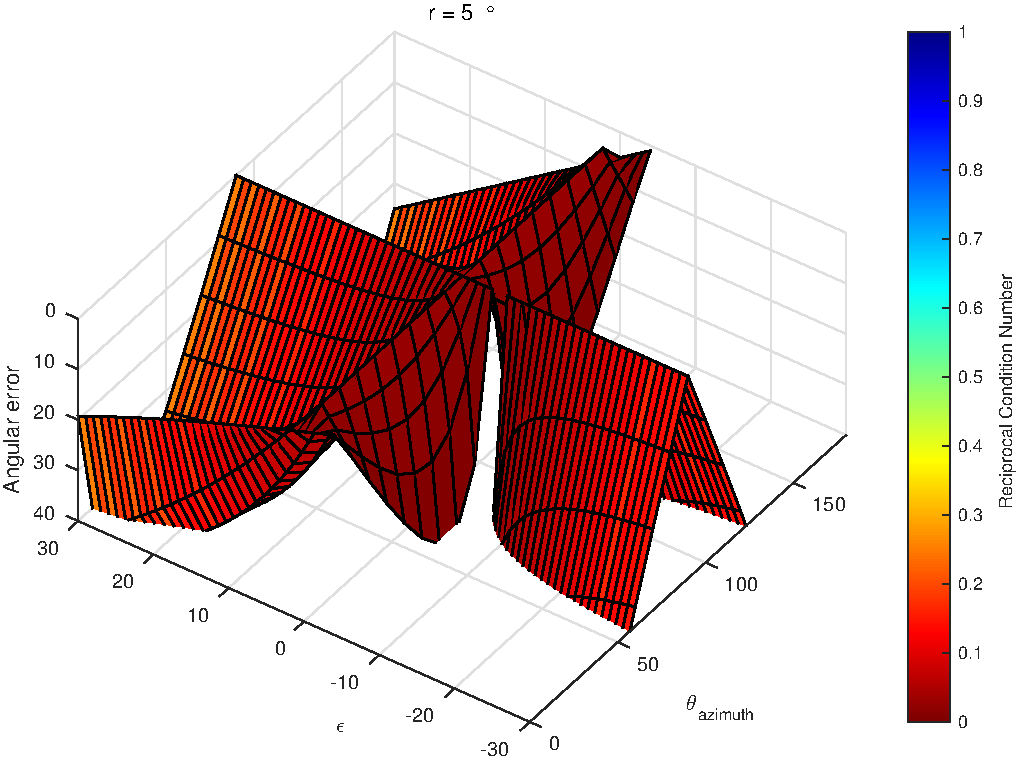
\includegraphics[width=0.45\linewidth]{q3_experiment_2a_view_1.pdf}
  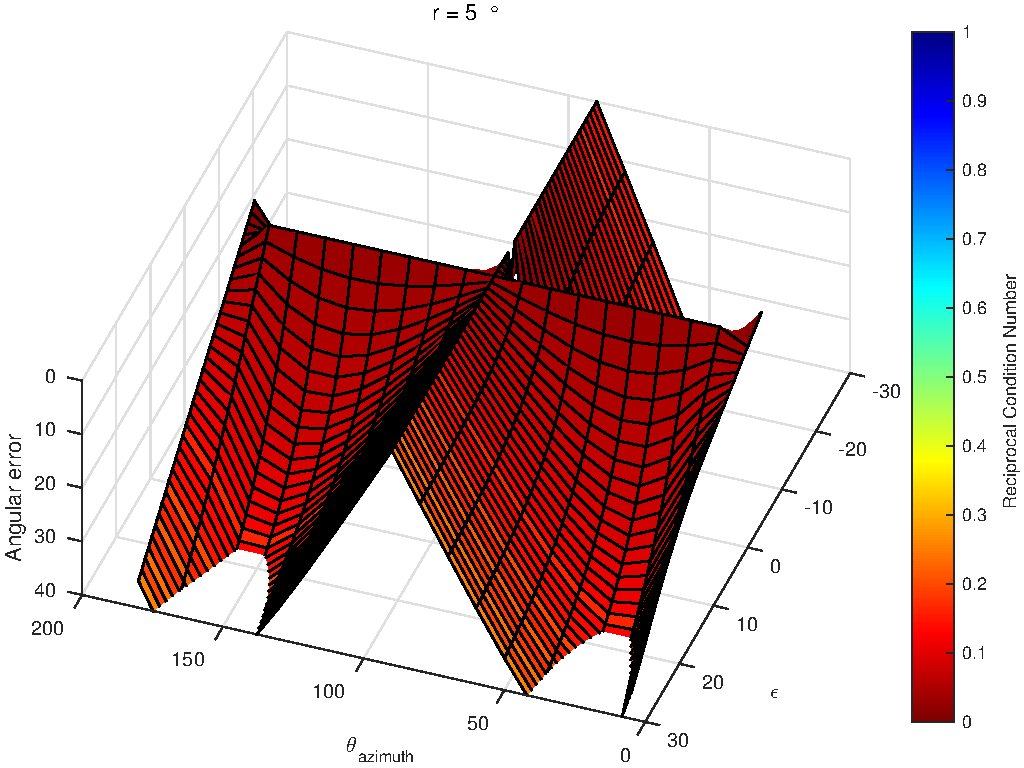
\includegraphics[width=0.45\linewidth]{q3_experiment_2a_view_2.pdf}
  \caption[Experiment 2 on a small lighting angle]
   {Same experiment as fig.~\ref{q3:exp2}, but with an lighting angle $r = 5\degree$. The missing section in the surface is when the error is $\epsilon_r = -5\degree$, meaning that the measure positioned all three light sources at the exact same location ($r = 0\degree$).}
  \label{q3:exp2a}
\end{figure}

\todo{DO WITH ANOTHER PLAN}

It is interesting to note from fig~\ref{q3:exp2} and \ref{q3:exp2a} that if a surface normal is pointing directly to the center of the triangle formed by the three lights, its recovery will always be correct, even in sub-optimal lighting condition. This is because the values of the three pixel intensities are always equal, making the ground truth the only possible solution to the linear system of equation. Furthermore, the reconstruction gives the right result when no error is applied ($\epsilon_r = 0\degree$), except when not all three light sources are shining on the surface (when $\theta_{\text{azimuth}}$ is near $0\degree$ or $180\degree$). In this particular problem, it is interesting to note that the most stable matrix won't necessarily result in the most accurate reconstruction, because of the systematic measurement error $\epsilon_r$. In this particular problem, as long as the three lighting sources are in line of sight with the target surface, the reconstruction angular error is a function of the ground truth surface normal and the lighting measurement error.

\todo{DEFINE X-Y-Z}

\FloatBarrier
\section{Question 4}

I will assume the reconstruction technique to analyze is photometric stereo. I will suppose that YHG666 has no atmosphere and that the captures are performed whenever the sun-like star is shining over the monolith surface (nighttime comprised). I will also assume that the black hole does not disturb the light rays coming from the sun-like star (no lighting curvature) and that its gamma rays are always perturbing the sensor equally (even if the black hole is not in direct line of sight with the CCD sensor).

I will suppose that YHG666 has no inclination, so the planar trajectory $\phi$ of the binary system (sun-like and black hole) is $90\degree$ minus the latitude of the immobile probe. If the planet had an inclination, the planar trajectory $\phi$ would be a combination of the latitude of the probe and the position of YHG666 with respect to the binary system (its day of the year). Furthermore, this inclination would create an angle of declination making the sun-like star not totally planar, as explained in~\cite{shen-pg-14}, improving the reconstruction performance when performed at another time than the equinoxes.

I will further suppose the monolith to be predominantly vertical. If the immobile probe is located in the northern hemisphere of the planet, the orientation of the flat surface to be reconstructed should be toward south to maximize the reconstruction performance. This ensures that the sun-like star shines upon the surface from dusk to dawn. For the same reason, if the probe landed in the southern hemisphere, the flat surface should be toward north. An example setup is shown in fig.~\ref{q4:setup}. Some possible trajectories of the binary system in the sky are shown in fig.~\ref{q4:trajectories}. For the rest of the answer, I will suppose the probe to have landed in the northern hemisphere.

\begin{figure}
  \centering
  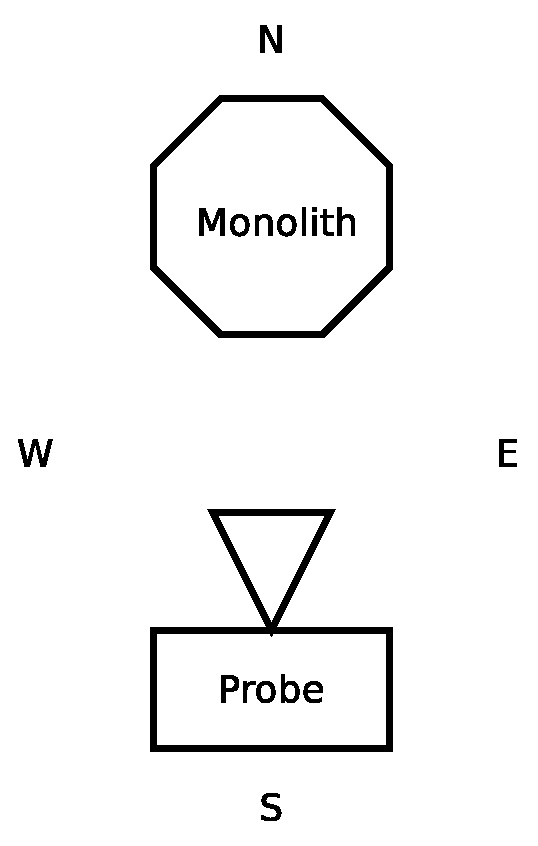
\includegraphics[width=0.2\linewidth]{q4_setup.eps}
  \caption[Experiment setup]
   {Top-down view of the experiment setup, assuming the immobile probe landed in the northern hemisphere. The $x$-axis is west-east, the $y$-axis is nadir-zenith (toward ``top'') and the $z$-axis is north-south toward the camera. }
  \label{q4:setup}
\end{figure}

\begin{figure}
  \centering
  \begin{tabular}{cc}
  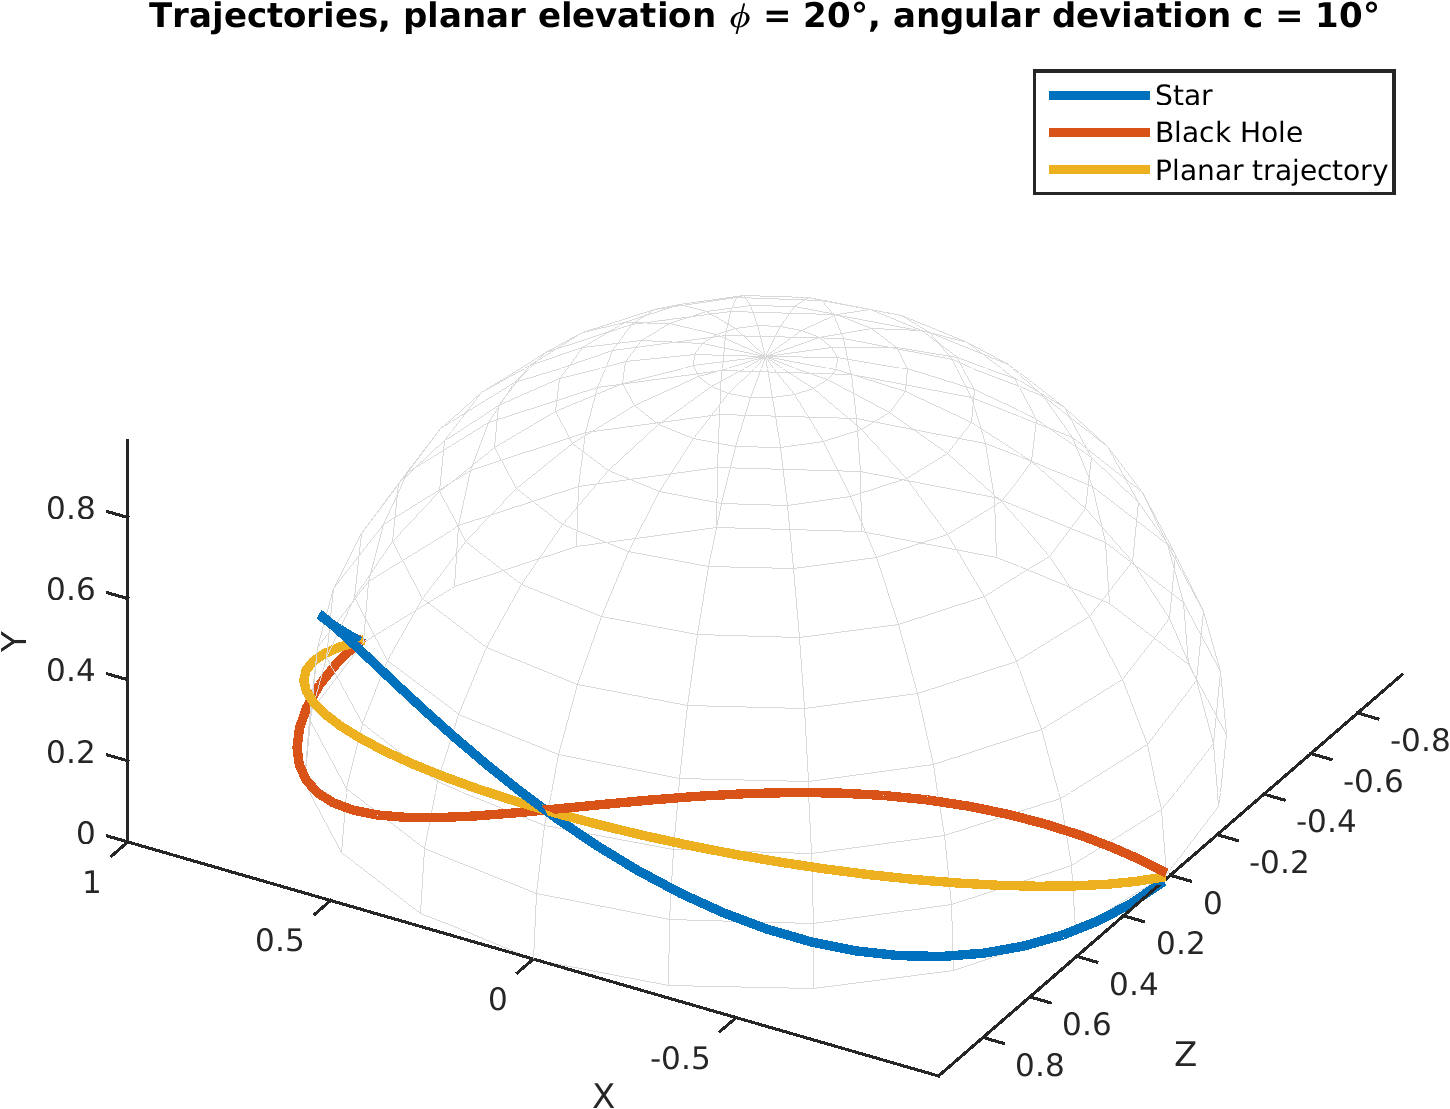
\includegraphics[width=0.45\linewidth]{q4_trajectory_el20_dev10.png} &
  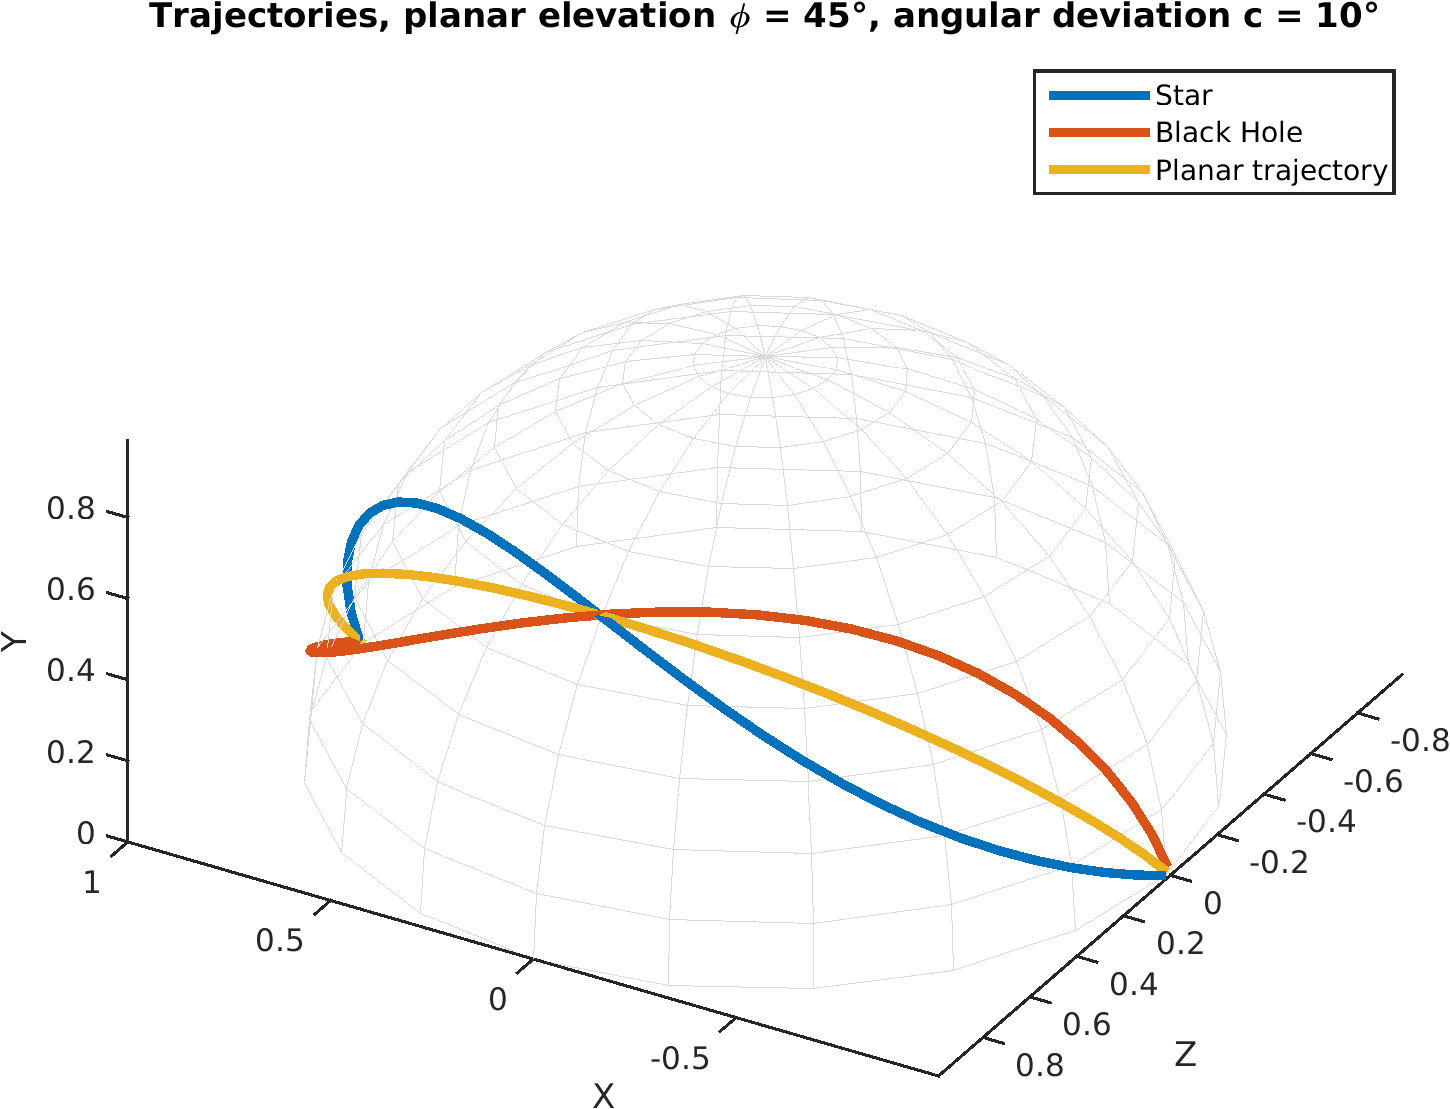
\includegraphics[width=0.45\linewidth]{q4_trajectory_el45_dev10.png} \\ \vspace{1em}
  (a) & (b) \\
  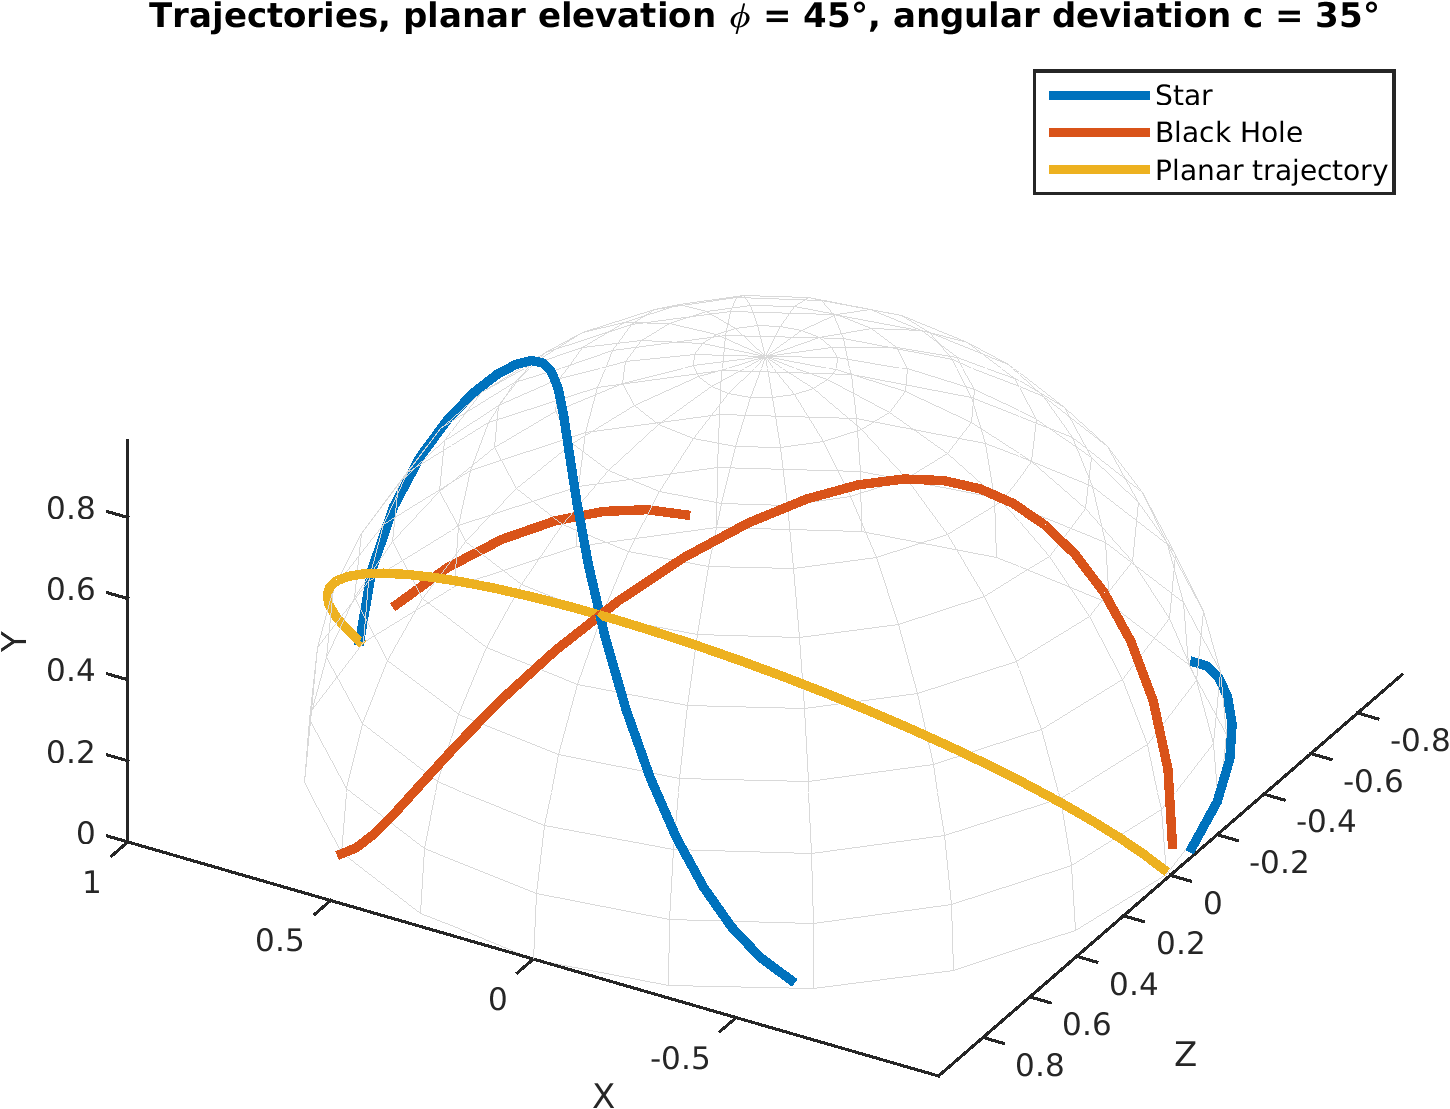
\includegraphics[width=0.45\linewidth]{q4_trajectory_el45_dev35.png} &
  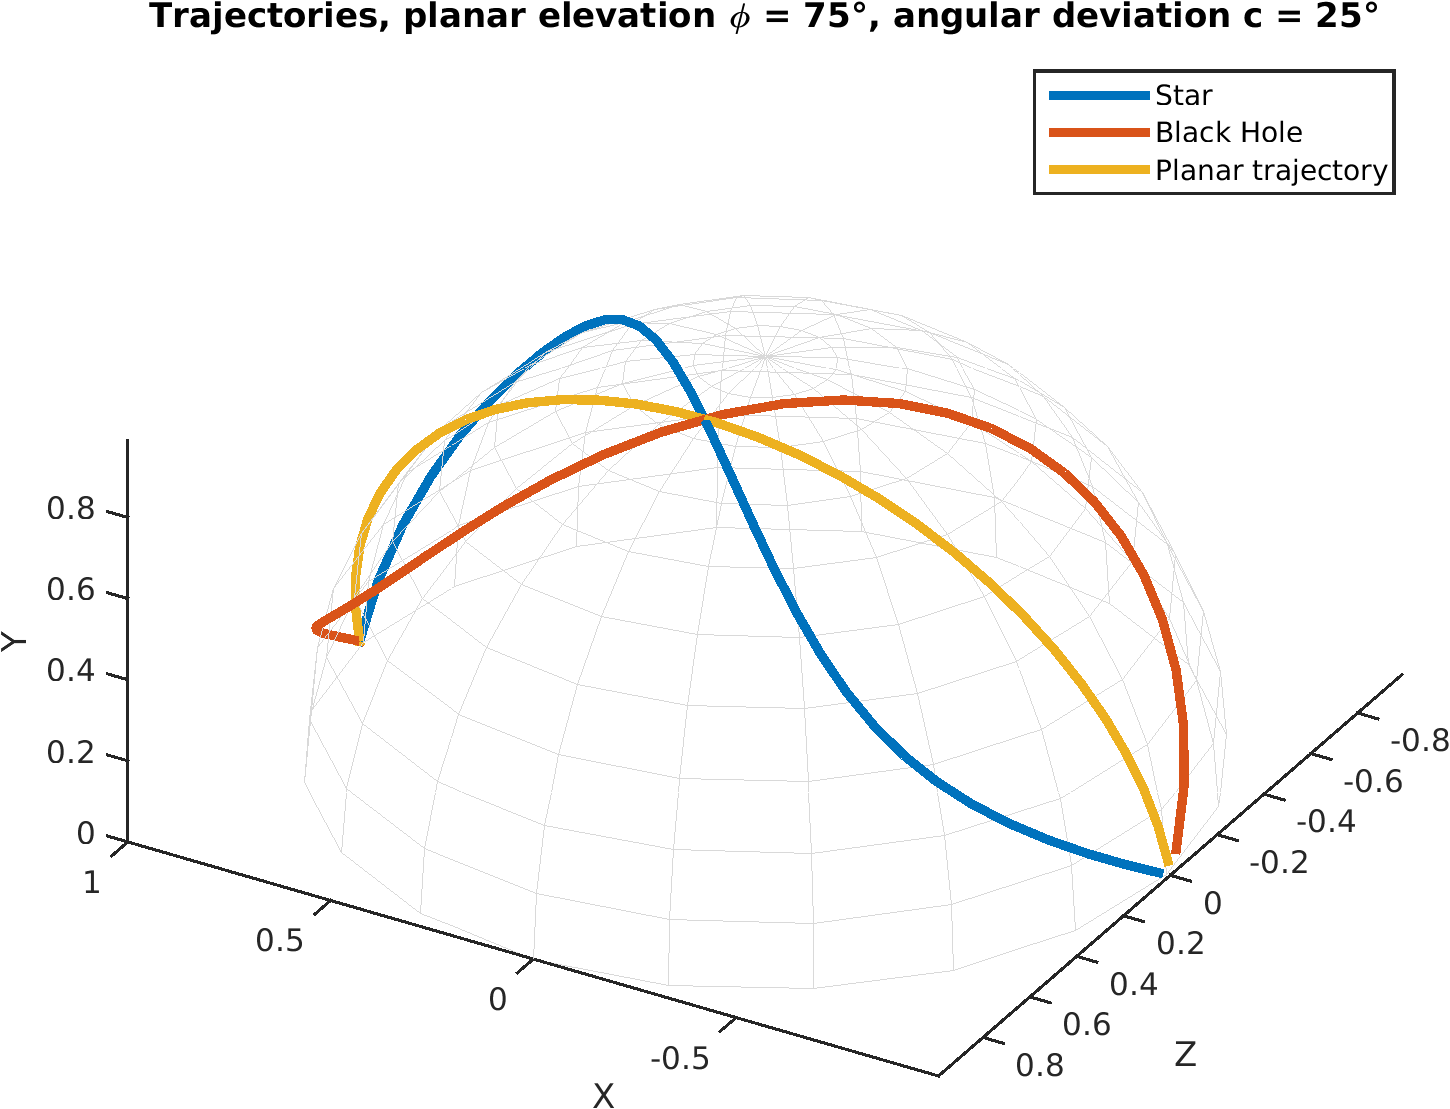
\includegraphics[width=0.45\linewidth]{q4_trajectory_el75_dev25.png} \\
  (c) & (d)
  \end{tabular}
  \caption[Example trajectories]
   {Example trajectories with various planar elevation $\phi$ and angular deviation $c$. (a) $\phi = 20\degree$, $c = 10\degree$, (b) $\phi = 45\degree$, $c = 10\degree$, (c) $\phi = 45\degree$, $c = 35\degree$, (d) $\phi = 75\degree$, $c = 20\degree$. Notice how the sun get visible again during nighttime when the angular deviation $c$ is high relatively to $\phi$, as in (c).}
  \label{q4:trajectories}
\end{figure}

Reconstructing a scene could be done optimally (in a least-squares sense) by performing
\begin{equation}
\hat{\B{n}} = \left( \B{L}^T\B{L}\right)^{-1} \B{L}^T \B{b}
\quad,
\end{equation}
where $b$ is the observed pixel intensities and $\left( \B{L}^T\B{L}\right)^{-1} \B{L}^T$ is the pseudoinverse of the lighting matrix $\B{L}$.
As defined in \cite{holdgeoffroy-3dv-15}, a 95\% confidence interval for a normal $\B{n}$ is given by
\begin{equation}
\hat{\B{x}} \pm \B{\delta} , \quad \text{with} \delta_k = 1.96\frac{\sigma_{\text{CCD}}}{\rho}\lambda_k
\quad,
\end{equation}
where $\sigma_\text{CCD}$ is the image noise, $\rho$ is the albedo of the surface and $\lambda_k$ is the square root of the $k$-th element on the diagonal of $\left(\B{L}^T\B{L}\right)^{-1}$~\cite{Hastie-09}.
Supposing the albedo to be constant, the uncertainty of the reconstruction can then be seen as the product of $\sigma_\text{CCD}$ and a conditioning marker $\lambda_k$. This $\lambda_k$ can be interpreted as a gain factor, amplifying the uncertainty due to the noise $\sigma_\text{CCD}$. First, I will explain the impact of the angular deviation $c$ on the stability of the reconstruction in terms of noise gain. Then, I will present simulations results taking into account the noise $\sigma_\text{CCD}$.

\begin{figure}
  \centering
  \begin{tabular}{ccc}
  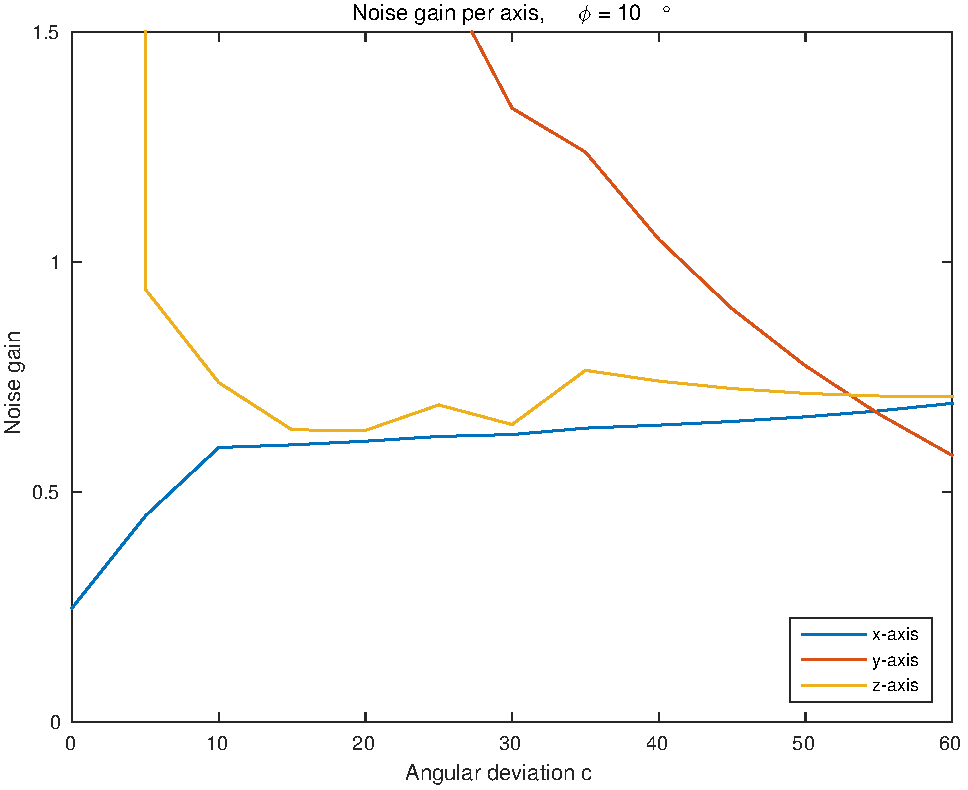
\includegraphics[width=0.30\linewidth]{q4_noise_10.pdf} &
  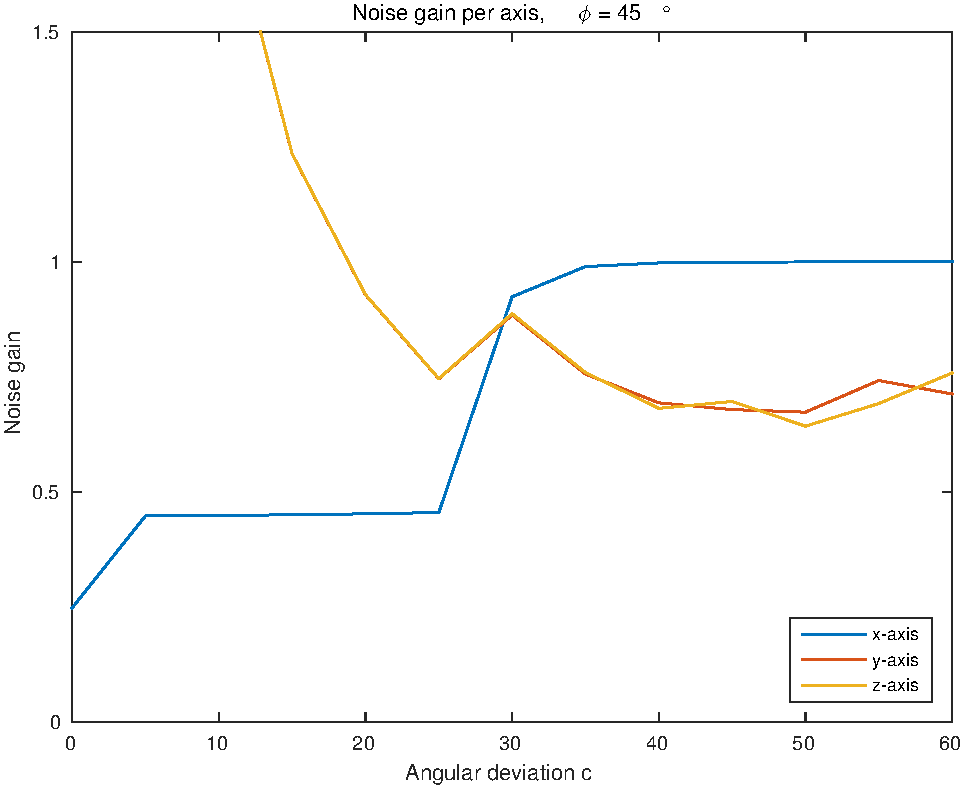
\includegraphics[width=0.30\linewidth]{q4_noise_45.pdf} &
  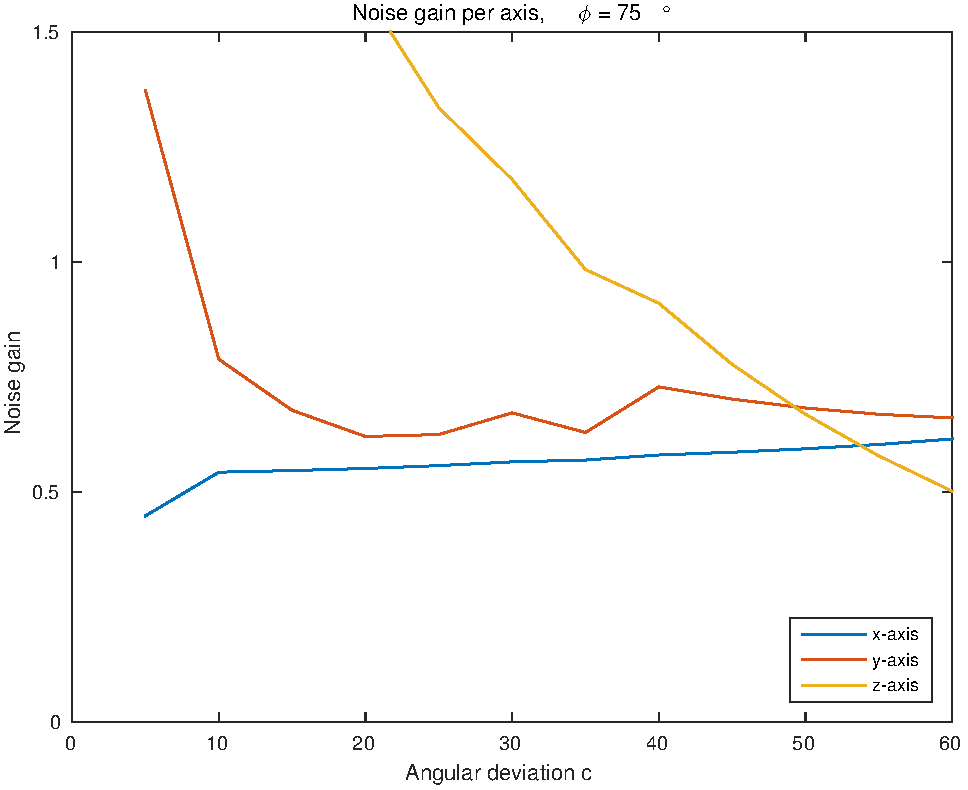
\includegraphics[width=0.30\linewidth]{q4_noise_75.pdf} \\
  (a) &
  (b) &
  (c)
  \end{tabular}
  \caption[Per-component noise amplification factor]
   {Noise amplification factor $\lambda_k$, per-component ($\lambda_x$ in blue, $\lambda_y$ in red and $\lambda_z$ in orange), as defined in fig.~\ref{q4:setup}.}
  \label{q4:lambda}
\end{figure}

A different noise gain $\lambda_k$ is applied to each of the 3D axes, namely $\lambda_x$, $\lambda_y$ and $\lambda_z$ for the $x$, $y$ and $z$-axis, respectively. For the current setup, these three noise gain factors are presented in fig.~\ref{q4:lambda}. It is worth noting that for small to medium deviation angles $c$, the noise gain for the $x$-axis is relatively small, whereas the two other components are large. This means that the $x$-axis component of the reconstruction is relatively certain, while the reconstruction is more uncertain on the $y$ and $z$-axis. This is coherent with the problem setup: a lot of information is present in the west-east axis, but the small angular deviation $c$ gives almost no information on the other axes (see \ref{q4:setup} for the axis definition). The abrupt slope around $c = 30\degree$ on the $x$-axis in fig.~\ref{q4:lambda} (b) is caused by the sun-like star falling under the horizon during the ``day'', making those capture times unusable, as the surface normal points toward south (see \ref{q4:trajectories} (c)).

The impact of the noise $\sigma_\text{CCD}$ on the reconstruction normal is shown in fig.~\ref{q4:recons_err}. For the three first figures (a-c), three different noise values were selected: 0.5\%, 1\% and 5\% over the total dynamic range of the image sensed. They represent respectively, very roughly speaking, the usual noise (on earth, without prominent noise source) of a top-of-the-line camera sensor (like a Nikon D5 or a Canon 1D), a good D-SLR and a pretty bad point-and-shoot camera. The others parameters (angular deviation $c$ and planar trajectory elevation $\phi$) were kept fixed for these three figures. The angular error distribution among for these figures is mostly similar. As predicted, the noise amplification factors $\lambda_k$ is multiplied by the sensor noise $\sigma_\text{CCD}$ to give the reconstruction error. If the amplification factors are constant (same angular deviation $c$ and planar trajectory elevation $\phi$), doubling the sensor noise would double the reconstruction error.

For fig.~\ref{q4:recons_err} (d-f), the noise $\sigma_\text{CCD}$ was set to $1\%$. For a different noise level, just multiply the $x$-axis of the histogram with the desired amount of noise. The general idea of these figures is that increasing the angular deviation $c$ improves the reconstruction performance, as a quick comparison of fig.~\ref{q4:recons_err} (d) and (e) can confirm. This is coherent with the noise gain analysis in fig.~\ref{q4:lambda}, where increasing the angular deviation $c$ yields a better overall reconstruction, where the uncertainty decreases for the $y$ and $z$-axis components. Only the $x$-axis increases, first insignificantly in (a) and (c) versus the gain brought by the other components. In (b), as explained previously, the sun-like star is lost below the horizon during the course of the day, generating the bump in the $x$-axis uncertainty.

The second variable influencing the reconstruction is the planar trajectory elevation $\phi$. Fig.~\ref{q4:recons_err} (f) has a slightly better reconstruction performance than (d), even if its angular deviation $c$ is smaller, simply because the planar trajectory elevation $\phi$ is better suited in this case. This effect can also be seen in fig.~\ref{q4:lambda} (a) where the $y$-axis component (the red line) is very uncertain until an angular deviation $c \approx 30\degree$ for a planar trajectory elevation $\phi = 10\degree$, whereas in (b) a planar trajectory elevation of $\phi = 45\degree$ yields pretty good overall certainty at $c \approx 20\degree$.

%Next time I plan to deploy an immobile probe on a planet, I will equip it with a polarizing filter. Since most light reflected by a non-metallic surface is polarized, it could help block some of the unwanted

\begin{figure}
  \centering
  \begin{tabular}{ccc}
  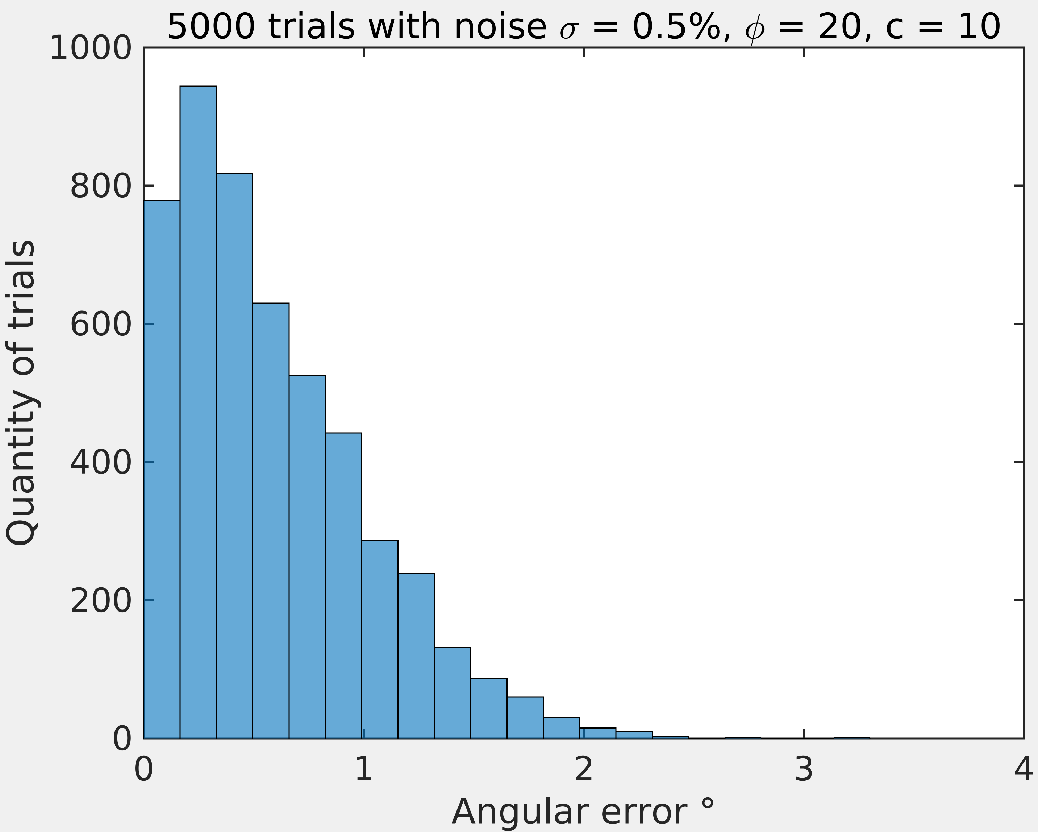
\includegraphics[width=0.30\linewidth]{q4_error_el_20_dev_10_noise_0_005000.pdf} &
  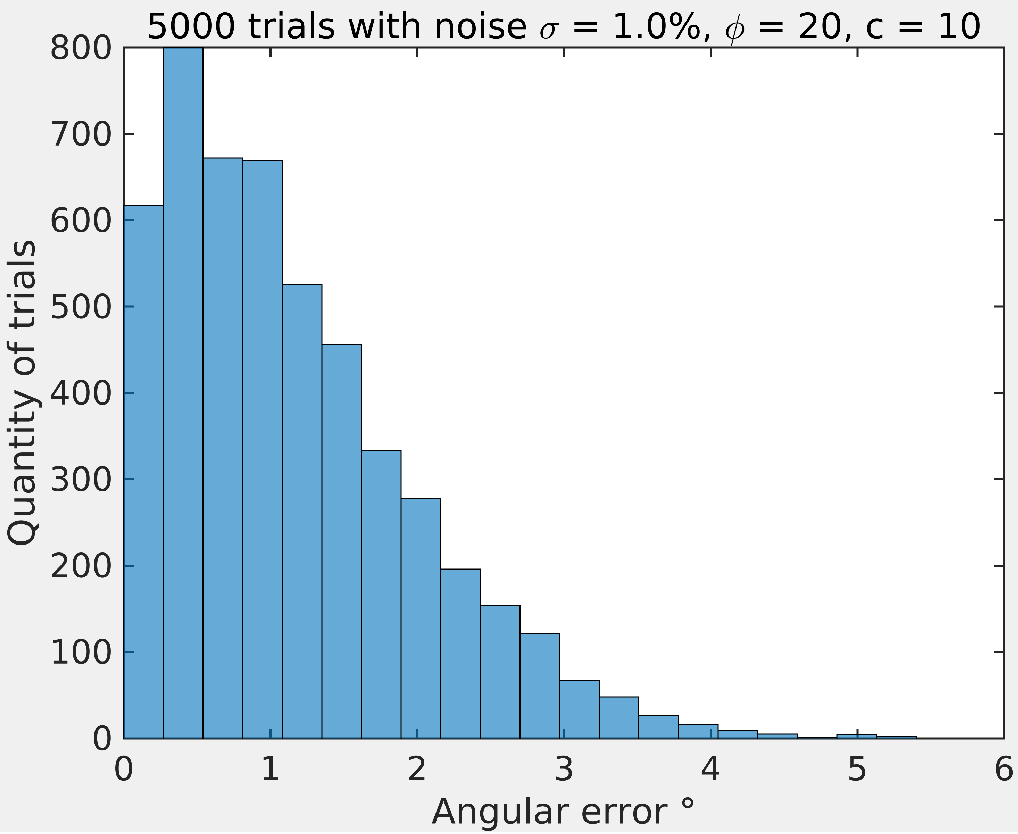
\includegraphics[width=0.30\linewidth]{q4_error_el_20_dev_10_noise_0_010000.pdf} &
  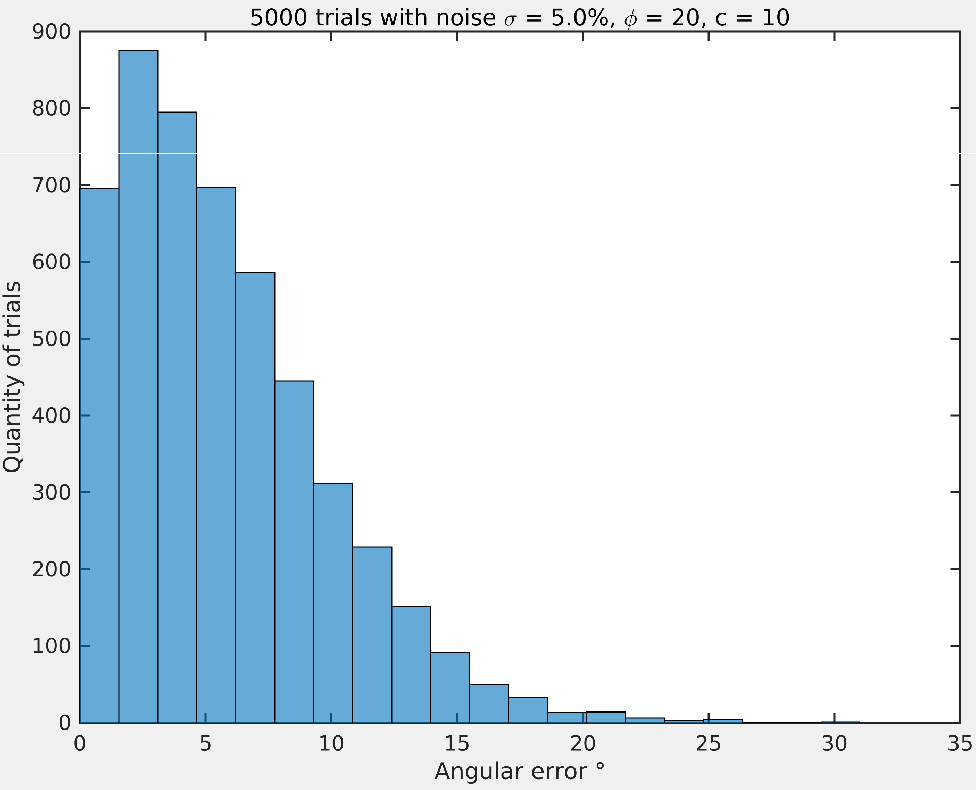
\includegraphics[width=0.30\linewidth]{q4_error_el_20_dev_10_noise_0_050000.pdf} \\
  (a) &
  (b) &
  (c) \\
  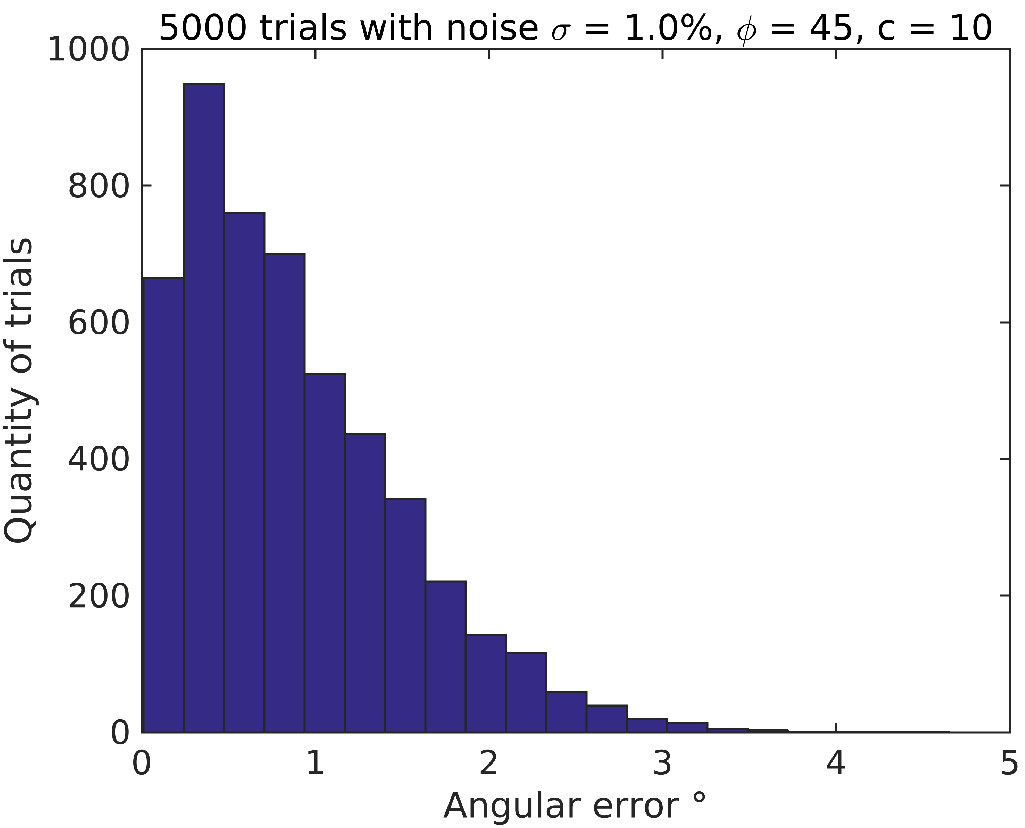
\includegraphics[width=0.30\linewidth]{q4_error_el_45_dev_10_noise_0_010000.pdf} &
  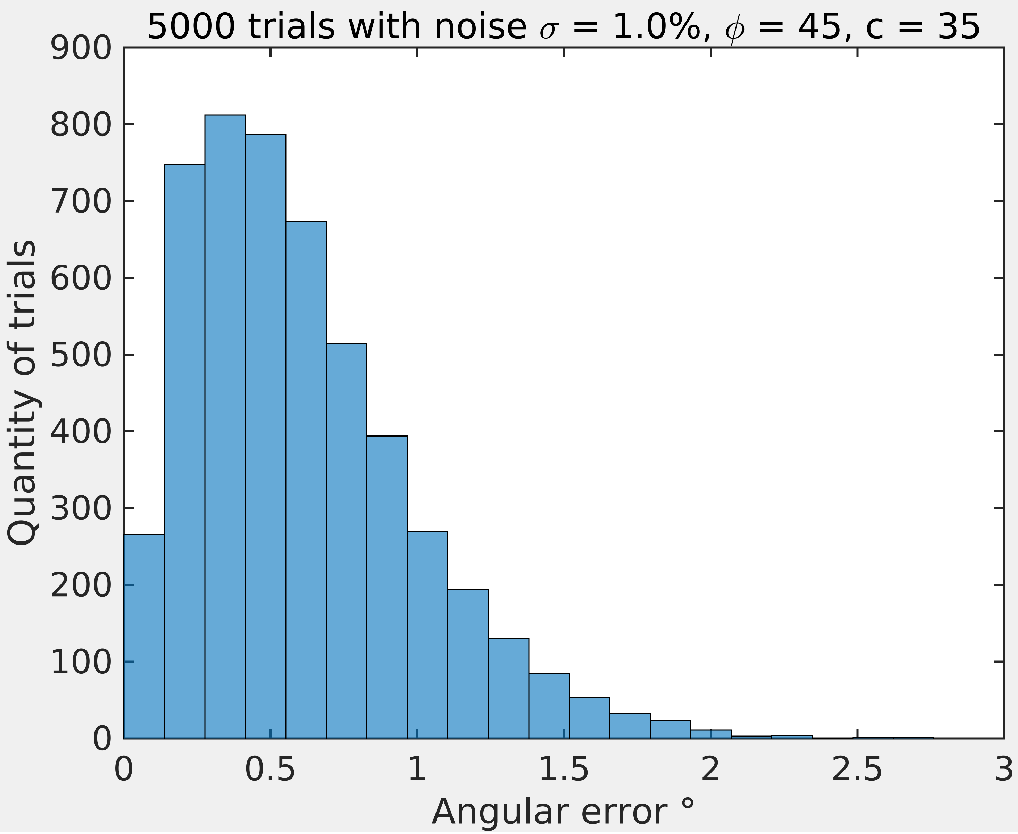
\includegraphics[width=0.30\linewidth]{q4_error_el_45_dev_35_noise_0_010000.pdf} &
  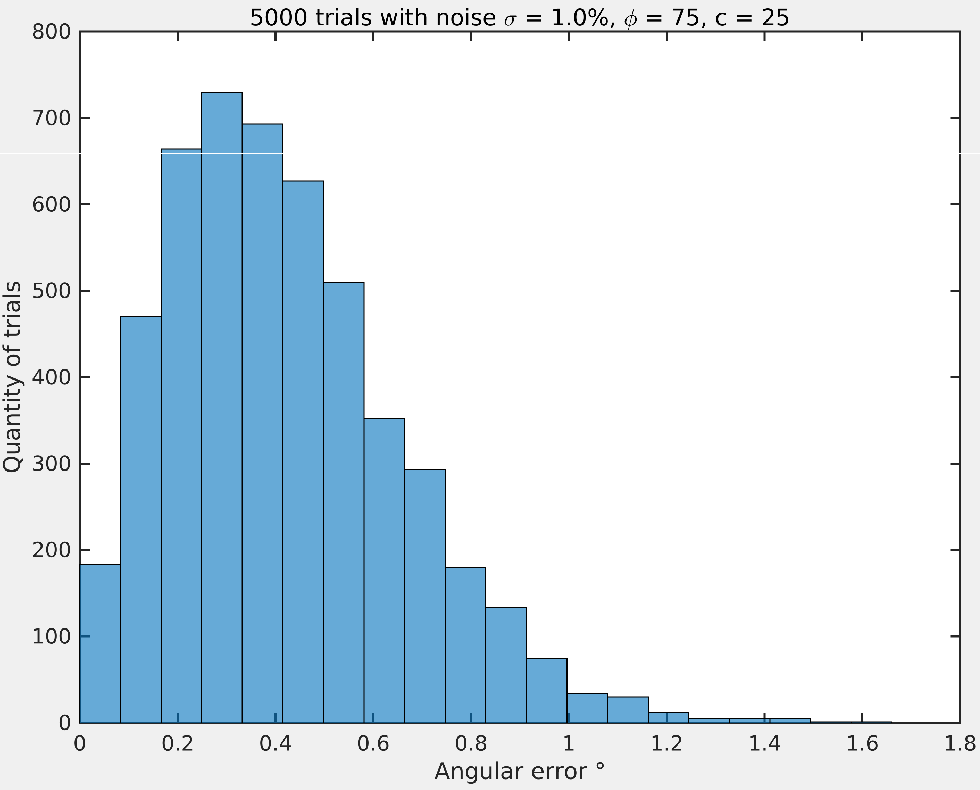
\includegraphics[width=0.30\linewidth]{q4_error_el_75_dev_25_noise_0_010000.pdf} \\
  (d) &
  (e) &
  (f) 
  \end{tabular}
  \caption[Reconstruction error with $\phi = 10\degree$.]
   {Reconstruction error for a planar trajectory $\phi = 10\degree$ for noise level $\sigma_\text{CCD} = 0.5\%$ (a), $1\%$ (b) and $5\%$ (c). As predicted, these three distributions are all very similar since the varying noise factor $\sigma_\text{CCD}$ is multiplied by a constant amplification factors $\lambda_k$.}
  \label{q4:recons_err}
\end{figure}

\chapter{Questions by Paulo Gotardo}

\section{Question 5}
\subsection{(a)}
\textbf{Let $\B{A} \in \mathbb{R}^{m \times n}$, with $m \gg n$. Show how the eigenvalues and (unit) eigenvectors of $\B{AA}^T$ can be obtained from the eigen decomposition of the smaller matrix $\B{A}^T\B{A}$.}

By the definition of the Singular Value Decomposition (SVD), any real matrix $\B{A}$ can be factored such as
\begin{equation}
\B{A} = \B{U \Sigma V}^T \quad.
\end{equation}
These matrices $\B{U}$, $\B{\Sigma}$ and $\B{V}$ are closely related to the eigen decomposition. First, $\Sigma$ is a diagonal matrix yielding the singular values of $A$, which are the square roots of the eigenvalues of both $\B{AA}^T$ and $\B{A}^T\B{A}$. Second, the columns of $\B{U}$ and $\B{V}$ are, by definition, the eigenvectors of $\B{AA}^T$ and $\B{A}^T\B{A}$, respectively. We can convince ourselves of both statements with these relations:
\begin{align*}
\B{AA}^T           &= \B{V\Sigma}^T\B{U}^T \; \B{U\Sigma V}^T
                        &&= \B{V\Sigma}^T\B{IU\Sigma V}^T 
                        &&&= \B{V\Sigma}^T\B{\Sigma V}^T \quad,\\
\B{A}^T\B{A}  &= \B{U\Sigma V}^T \; \B{V\Sigma}^T\B{U}^T
                        &&= \B{U\Sigma V}^T \; \B{V\Sigma}^T\B{U}^T
                        &&&= \B{U\Sigma}\B{\Sigma}^T\B{U}^T \quad.
\end{align*}
As the columns of $\B{U}$ and $\B{V}$ are a orthonormal basis (as they hold the eigenvectors), both $\B{U}^T\B{U}$ and $\B{V}^T\B{V}$ result in the identity matrix $\B{I}$.

Two relationships are sought in the question: the eigenvalues and eigenvectors of both pre and post multiplication by the transpose. First, the relationship between the eigenvalues of $\B{A}^T\B{A}$ and $\B{AA}^T$ is pretty simple: they are the same. On the other hand, their eigenvectors are only related through $\B{A}$:
\begin{align*}
\B{A}  &= \B{U \Sigma V}^T \\
\B{AV} &= \B{U \Sigma V}^T \B{V} = \B{U \Sigma I} \\
\B{AV\Sigma}^\dagger &= \B{U \Sigma \Sigma}^\dagger = \B{U} \quad,
\end{align*}
where $\B{\Sigma}^\dagger$ is the pseudoinverse of $\B{\Sigma}$. This $\B{\Sigma}^\dagger$ is used as a normalization factor for the $\B{AV}$ matrix; normalizing each column of $\B{AV}$ would produce the same result.

This relation will provide as many eigenvectors as there are linearly independent vectors of $\B{AA}^T$. Since $m \gg n$, this means that at most $n$ eigenvectors of $\B{AA}^T$ will be found. The rest of the resulting matrix will contain only zeros. The vectors that are missing span the null space of $\B{A}^T$ (and $\B{AA}^T$).

\subsection{(b)}

Performing optimization using a $L_1$-norm loss function, sometimes called a least absolute deviations (LAD), is quite different in practice from using a least squares ($L_2$-norm loss function). While the LAD is more robust that least squares, meaning that it is more resistant to outliers in the data, it is also more unstable, meaning that a small change in a single data point can potentially change the solution a lot. Furthermore, a main major difference is that while least square allows only a single optimal solution, LAD allows multiple solutions to be equivalent. An example of this phenomenon can be visualized in fig.~\ref{q5b:paths}.

\begin{figure}
  \centering
  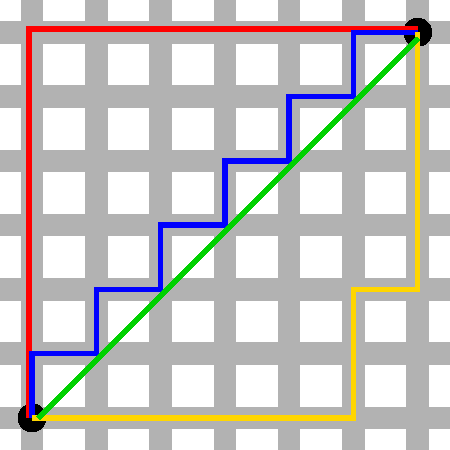
\includegraphics[width=0.45\linewidth]{q5b_manhattan_distance.pdf}
  \caption[ Examples of $L_1$ and $L_2$ distances ]
   {The distance between two black dots is shown in $L_1$ (red, blue and yellow) and $L_2$ (green) space. Note that while there is only one optimal solution in $L_2$, there are many possible optimal solutions in $L_1$ which yield the same $L_1$ distance. Image under public domain license from Wikimedia Commons.}
   \label{q5b:paths}
\end{figure}

As such, least squares can be solved directly in a linear system of equation by taking the (pseudo-)inverse of the matrix. But LAD needs linear programming to be solved, as the constraints it poses may lead to multiple solutions. Fortunately, this problem is a convex, simplifying a great deal the strategies applying to it. Unfortunately, this loss function is not strictly differentiable, making gradient descent methods more difficult to apply.

One way to compute this is by performing an iterative method. Suppose the problem is written in matrix form
\begin{equation}
\B{x}^* = \arg \min_{\B{x}} \| \B{b} - \B{A}^T\B{x} \|_1 \quad, \B{x} \in \mathbb{R}^m
\quad,
\end{equation}
Then, one can propose this algorithm to solve the problem:
\begin{enumerate}
  \item Let $e_i^{(0)}$ = 0, and $k = 0$;
  \item Compute $\B{x}^{(k+1)} = \arg \min_{\B{x}} \B{Ax}^{(k)} - b - e$;
  \item Compute $e_i^{k} = \B{Ax}^{(k+1)} - \B{b}$;
  \item Let $k = k + 1$;
  \item Repeat the three last steps until convergence.
\end{enumerate}

One way to get around this is to perform soft-thresholding. A soft-thresholding function is defined as such:
\begin{equation}
\Phi(x) = 
\begin{cases}
  x + \lambda & \text{if } x\leq -\lambda \\ 
  0           & \text{if } -\lambda < x < \lambda \\
  x - \lambda & \text{if } x\geq \lambda
\end{cases}
\quad.
\end{equation}
\todo{validate}
The general appearance of this function is shown in fig.~\ref{q5b:soft-thresh}.

\begin{figure}
  \centering
  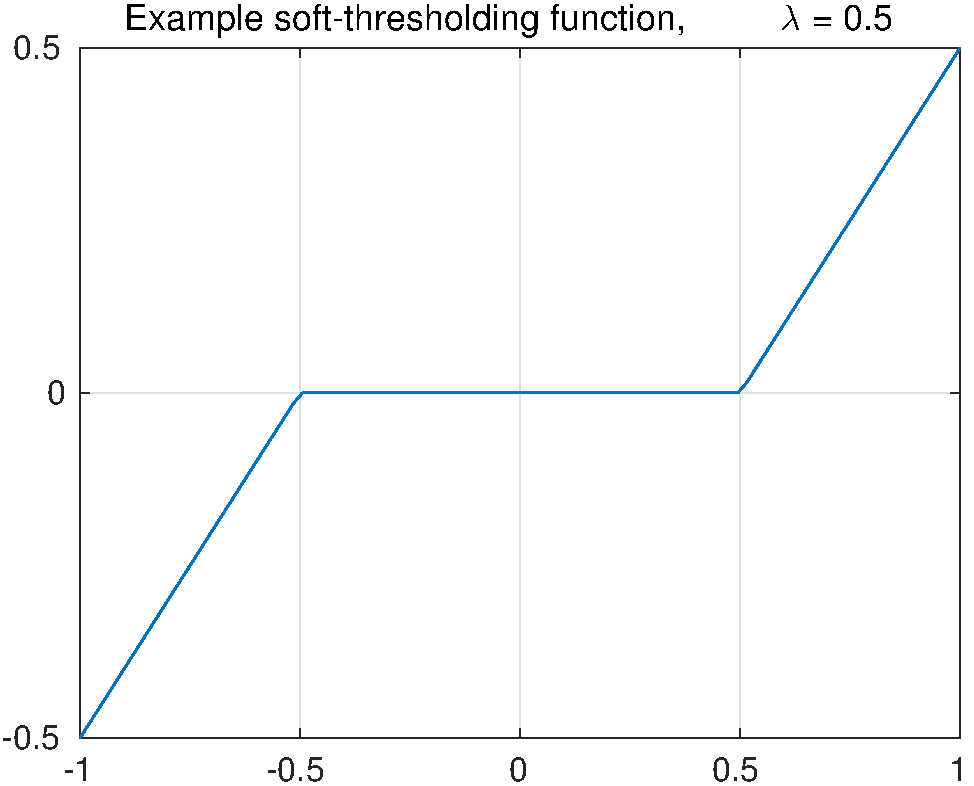
\includegraphics[width=0.45\linewidth]{q5c_soft_threshold_example.pdf}
  \caption[ Example soft-thresholding function ]
   {Example of soft-thresholding function, with $lambda = 0.5$.}
  \label{q5b:soft-thresh}
\end{figure}


[An example of an algorithm employing the soft-thresholding is explained by \cite{Kowalski2015}.]
\begin{equation}
\Phi \left(  \right)
\quad,
\end{equation}



\subsection{(c)}

The problem is a least squares minimization. It is a generalization of the core of photometric stereo, where a given pixel intensity $b$ for an image $i$ is explained by the multiplication of the light rays $\B{\omega}_j$ by the normal $\B{x}$ of a surface. The $\max$ ensures that light rays under the surface does not contribute to the pixel intensity.

An optimization strategy could be thought as the standard least squares sense.
[sensitive to outliers] [Multiple similar values will drive the solution towards them.]

Another could be using the result from (b).

\section{Question 6}

Temporally-multiplexed Photometric Stereo employs captures at different times yielding different lighting directions. This means that each row of the lighting matrix $\B{L}$ are taken at a different time, when the scene's lighting conditions changed. Contrarily, as \cite{Fyffe2011} puts it, ``In Spectrally-multiplexed photometric stereo, a scene is illuminated by multiple spectrally distinct light sources, and photographed by a camera system configured to capture multiple spectrally distinct color channels.'' In their work, they propose to divide the light spectrum in two using the Dolby\textsuperscript{\textregistered} dichroic filters, both having some non-overlapping red, green, and blue in their response spectrum.

Typically, PS is performed on pixel intensities, also called the luminance $y_i$ of a pixel $i$. This luminance can be expressed as a weighted sum of each pixel components, red $r_i$, green $g_i$ and blue $b_i$. The coefficients of the weighted sum depends on the colorspace used and on the measure (e.g.\ energy or perception). The two main luminance conversion functions are based on the CIE 1931 colorspace, $y_i = 0.2126r_i + 0.7152g_i + 0.0722b_i$ and its perceptually based counterpart, $y_i = 0.299r_i + 0.587g_i + 0.114b_i$. This conversion to luminance can be problematic when analyzing natural illumination, though. Most of the energy in natural illumination, aside from the small sun in the sky, is contained in the blue channel (as the sky is blue). However, this particular channel gets weighted down the most, as the blue channel coefficient is the lowest ($0.0722$ or $0.114$ in the earlier examples), making its impact on luminance much less than the other channels. To mitigate this issue, sophisticated channel fusion techniques have been proposed (e.g.\ \cite{jung-cvpr-15}), but this approach is clearly not a panacea to the problem.

This is where temporally-multiplexed outdoor photometric stereo can benefit from the color spectrum. To prevent the loss of information of merging the color channels together, \cite{johnson-cvpr-11} proposes to take each color channel as different captures, yielding different light sources. They argue that the information contained in every color channel of an image lit by natural illumination is enough in most cases to bring new constraints to the PS problem, helping the reconstruction. Hence, every picture taken could fill 3 rows of the $\B{L}$ matrix, one row per channel. This works because natural illumination is complex and may yield sensibly different lighting vectors for each channel. Cloud occlusion could possibly shift the color of the sun, sending the mean light in different directions depending on its wavelength.

While using spectral cues in temporally-multiplexed photometric stereo is worth investigating, it is far from being trivial to incorporate in general. For example, \cite{johnson-cvpr-11} supposed a constant albedo over the whole reconstructed surface in order to make their algorithm work. \cite{Fyffe2011} made the idea work on more generic surfaces, but used dichroic filters instead of simply using the three channels of a common camera, making the capture apparatus more complex. It is nevertheless an interesting idea to explore when performing further analysis on photometric stereo.
%\cite{MacDonald-2007}.

\section{Question 7}

Such an algorithm is presented in~\cite{Granados2010a}. The goal is to estimate, as best as possible, the irradiance $X_i$ of each pixel $i$. This is done by merging images of different exposures $j$ together. Basically, the proposed algorithm is as follows:
\begin{enumerate}
  \item{Acquire dark frames for all exposures values $e_j$;}
  \item{Assume constant variances $\hat{\sigma}_{X_j}^2{}^{(0)}$}
  \item{Compute the maximum likelihood estimate $\hat{\mu}_X^{(j)}$ for each pixel irradiance taking into account $\hat{\sigma}_{X_j}^2{}^{(j-1)}$;}
  \item{Estimate the pixel variances $\hat{\sigma}_{X_j}^2{}^{(j)}$ taking into account $\hat{\mu}^{(j-1)}$;}
  \item{Repeat the two previous steps until convergence;}
  \item{Smooth the final maximum likelihood estimate $\hat{\mu}_X$ according to the pixel variances $\hat{\sigma}_{X_j}^2$}.
\end{enumerate}

The optimal weighting function $w_{\mathrm{opt}}\left(v_j\right)$ of every pixel intensity $v_j$ is the reciprocal of the pixel variances $\frac{1}{\hat{\sigma}_{X_j}^2}$.

This algorithm is based on the idea that the pixel $i$ on an image of given exposure $j$ has an irradiance $X_{ij}$ related to the according to the pixel intensity $V_j$, its related dark frame $B_j$, the exposure time $t_j$ and the camera gains $g$ (global) and $a_i$ (non-uniform, pixel-dependent) as such:
\begin{equation}
\label{q7:eqirr}
X_{ij} \approx \frac{V_{ij} - B_{ij}}{t_j \cdot g \cdot a_i}
\quad.
\end{equation}

Two types of noise is taken into account in this analysis: the thermal noise and spatial noise. In the first category fall the photon shot noise, accounting the uncertainty of photons arrival, the dark current shot noise, accounting for electron movement not caused by incoming photons, and the readout noise, explaining the noise and imprecision in the electronic circuit producing the output digital values. The second category, spatial noise, regroup photo-response non-uniformity, accounting for variability in gain over the various pixels, and the dark current non-uniformity, accounting for dark current variability across the sensor surface due to temperature differences.

The output digital value $V_{ij}$ of a pixel $i$ on image $j$ is related to the irradiance it received $X_{ij}$ by the exposure time $t_j$, the dark current $D_i$, the readout noise $N_R$ and sensor gains $g$ and $a_i$ as such:
\begin{equation}
V_{ij} = \left[ g \cdot \left( t_j \left( a_i X_i + D_i \right ) + N_R\right) \right] \quad,
\end{equation}
where $\left[ \cdot \right]$ is the rounding operator. The variance of this pixel output value is
\begin{equation}
\label{q7:noisevariance}
\sigma_{V_{ij}}^2 = g^2 \sigma_{E_{ij}}^2 + \sigma_R^2
\quad,
\end{equation}
where $\sigma_{E_{ij}}^2$ is the photon shot noise and dark current shot noise combined, and $\sigma_R^2$ the readout noise, including the quantization error.

Plugging the pixel output variance described in equation~\eqref{q7:noisevariance} into the irradiance equation~\eqref{q7:eqirr}, we get:
\begin{equation}
\sigma_{X_{ij}}^2 = \frac{\sigma_{V_{ij}}^2 + \sigma_{B_{ij}}^2}{t_j^2 g^2 a_i^2} \quad.
\end{equation}

Until now, this analysis takes into account a single image. When merging the images together to form a HDR restoration, the variance due to noise becomes:
\begin{equation}
\sigma_{\mu_{X_{ij}}}^2 = \frac{1}{\sum_{j \in S_i} \frac{t_j^2 g^2 a_i^2}{g^2 t_j \left( a_i \mu_{X_i} + 2 \mu_{D_i} \right) + 2 \sigma_R^2}} \quad,
\end{equation}
when taking into account the set of images $S_i$ at pixel $i$.

If we suppose a simpler model with standard Gaussian noise $\mathcal{N}(0,\sigma_j^2)$ instead, the overall noise when using an optimal fusion algorithm such as the one described previously is
\begin{equation}
\sigma_{\mu_{X_{ij}}}^2 = \frac{1}{\sum_{j \in S_i} \frac{1}{\sigma_j^2}}
\quad,
\end{equation}
where $\sigma_j^2$ is proportional to $X_i$.

Its implications to photometric stereo are multiple. First, having better HDR environment maps allows a better estimation of the lighting shining over a given surface, improving the estimation of the lighting matrix $\B{L}$. Second, when using HDR object pictures, this would improve the accuracy of every pixel intensity $b_i$. Finally, a better noise model allows us to understand where lies the uncertainty in the reconstruction, which 3D axis is uncertain and where should we inject more priors (i.e.\ regularization) or where should we rely on a different technique to improve the reconstruction of a particular portion of surface or an uncertain component of the surface normal.

\chapter{Questions by Jean-François Lalonde}

\section{Question 8}
\subsection{(a)}
\textbf{Given a known lighting environment map $\B{L}$ (e.g.\ in latitude-longitude representation), explain how SH coefficients $s$ can be estimated from $\B{L}$.}

Each SH coefficients $s$ is linked to a basis function of degree $n$ and order $m$ defined over the sphere. Because these basis functions are orthogonal, the coefficients are computed by projecting the environment map $\B{L}$ on the according basis function, called $Y_n^m$:
\begin{equation}
s_n^m = \oiint\limits_{\Omega} \B{L}\left(\B{\omega} \right) Y_n^m \left( \B{\omega} \right) \mathrm{d} \B{\omega}   \quad.
\end{equation}
This formulation produces the least-squares fit of the basis functions over the environment map $\B{L}$.

In the discrete case, just like the environment map $\B{L}$, these functions can be represented in latitude-longitude representation. This allows the projection to be performed as the summation of its pixelwise multiplication with the environment map $\B{L}$:
\begin{equation}
s_n^m = \sum_{v=0}^{h} \sum_{u=0}^{w} \B{L}_{u,v} Y_n^m\left(u, v\right) \omega_{u,v}^2 \quad,
\end{equation}
for an environment map $\B{L}$ of width $w$ and height $h$. The solid angle subtended by pixel $u,v$, called $\omega_{u,v}$, is required to weight accordingly each pixel of both maps. Because of the latitude-longitude representation, each pixel covers a different surface area over the sphere. Multiplying each pixel by its solid angle weights them accordingly, ensuring that no pixel is more important than another one. The first 4 degrees of spherical harmonics real and imaginary bases are shown in fig.~\ref{q8a:sh_ex}.

Simply put, a given spherical harmonic coefficient---say $s_3^2$---is computed by doing
\begin{equation}
s_3^2 = \sum \underbrace{\begin{minipage}{84pt}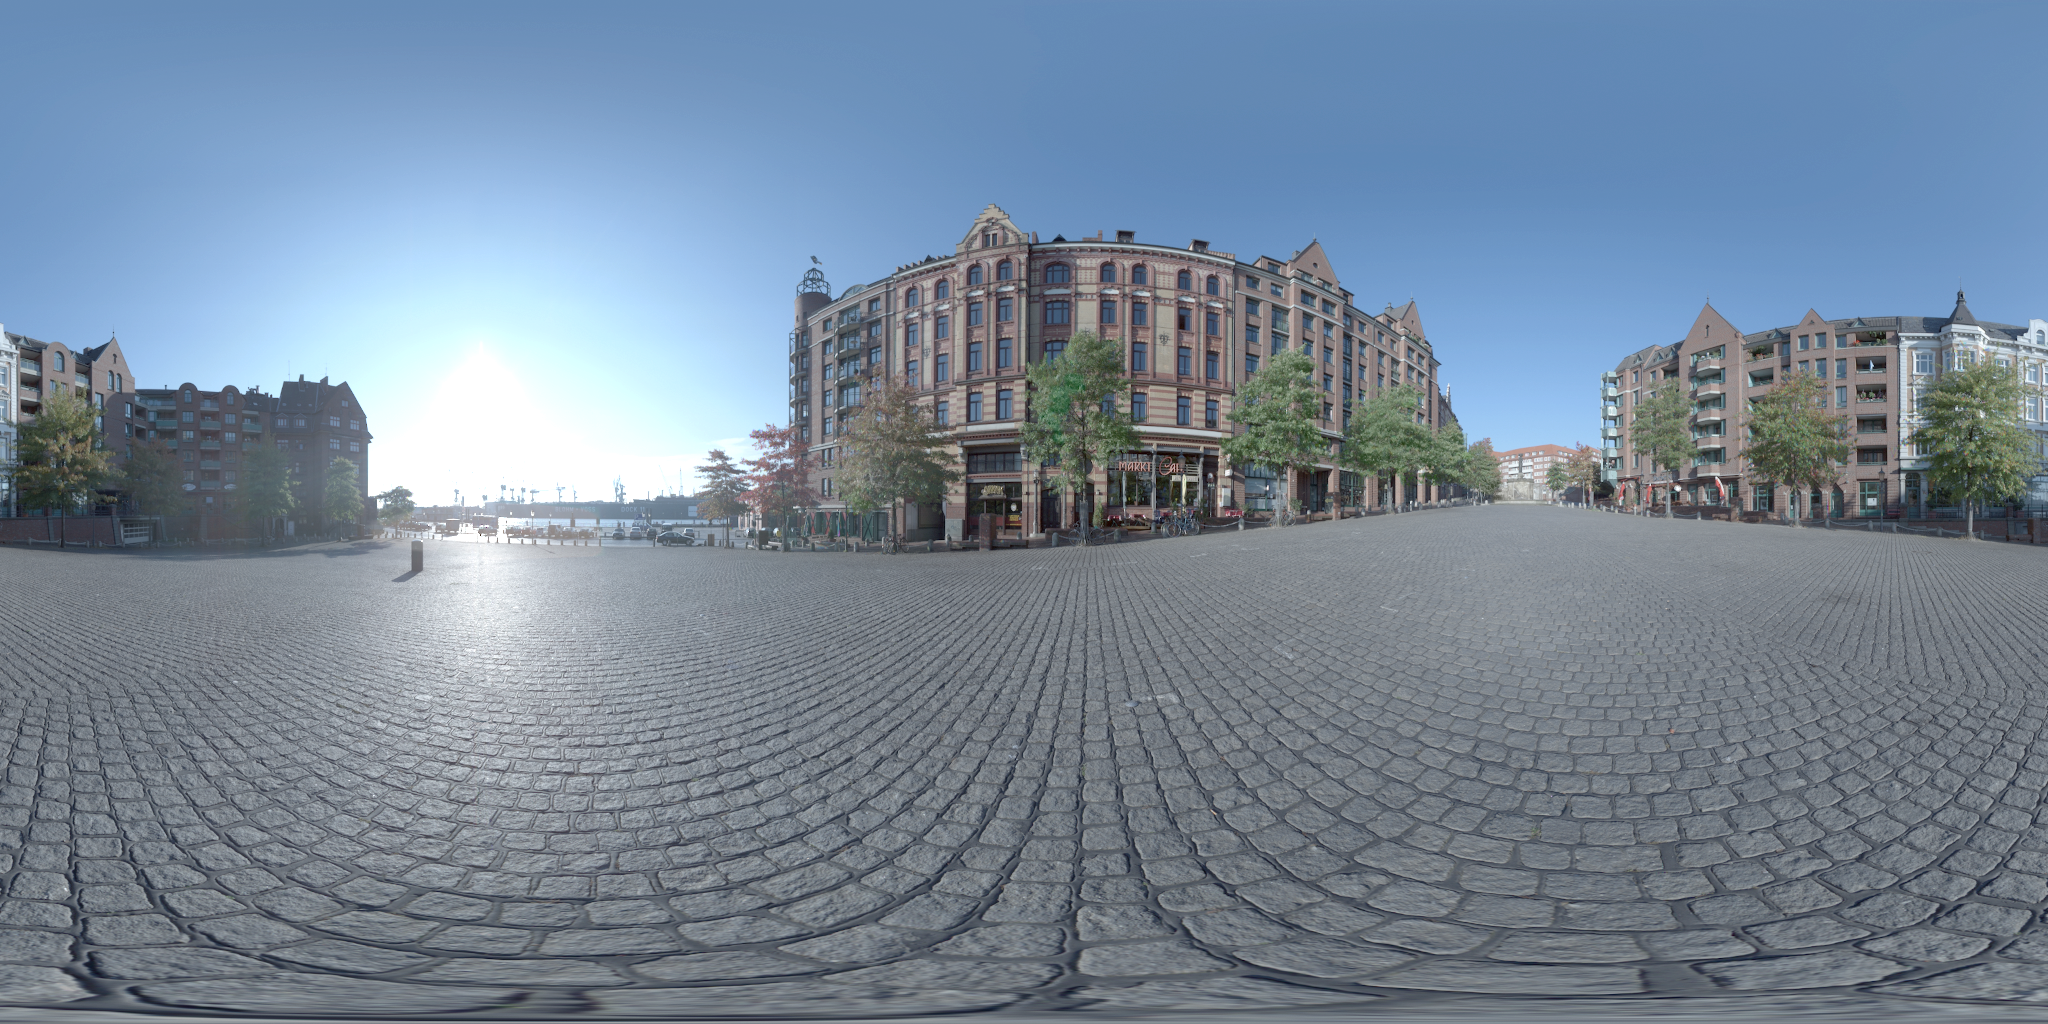
\includegraphics[height=42pt,width=84pt]{q8_envmap.png}\end{minipage}}_{\text{Environment map}} \cdot
\left(
\underbrace{\begin{minipage}{84pt}
\includegraphics[height=42pt,width=84pt]{q8_basis_3_2_real.png}\end{minipage}}_{\mathrm{Re}(Y_3^2)} + 
\underbrace{\begin{minipage}{84pt}
\includegraphics[height=42pt,width=84pt]{q8_basis_3_2_imag.png}\end{minipage} \; i}_{\mathrm{Im}(Y_3^2)}
\right)
\cdot
\left(
\underbrace{\begin{minipage}{84pt}
\includegraphics[height=42pt,width=84pt]{q8_solidangle.png}\end{minipage}}_{\text{Solid Angle}}
\right)^2
\quad.
\end{equation}


\begin{figure}
  \centering
  \begin{tabular}{cc}
  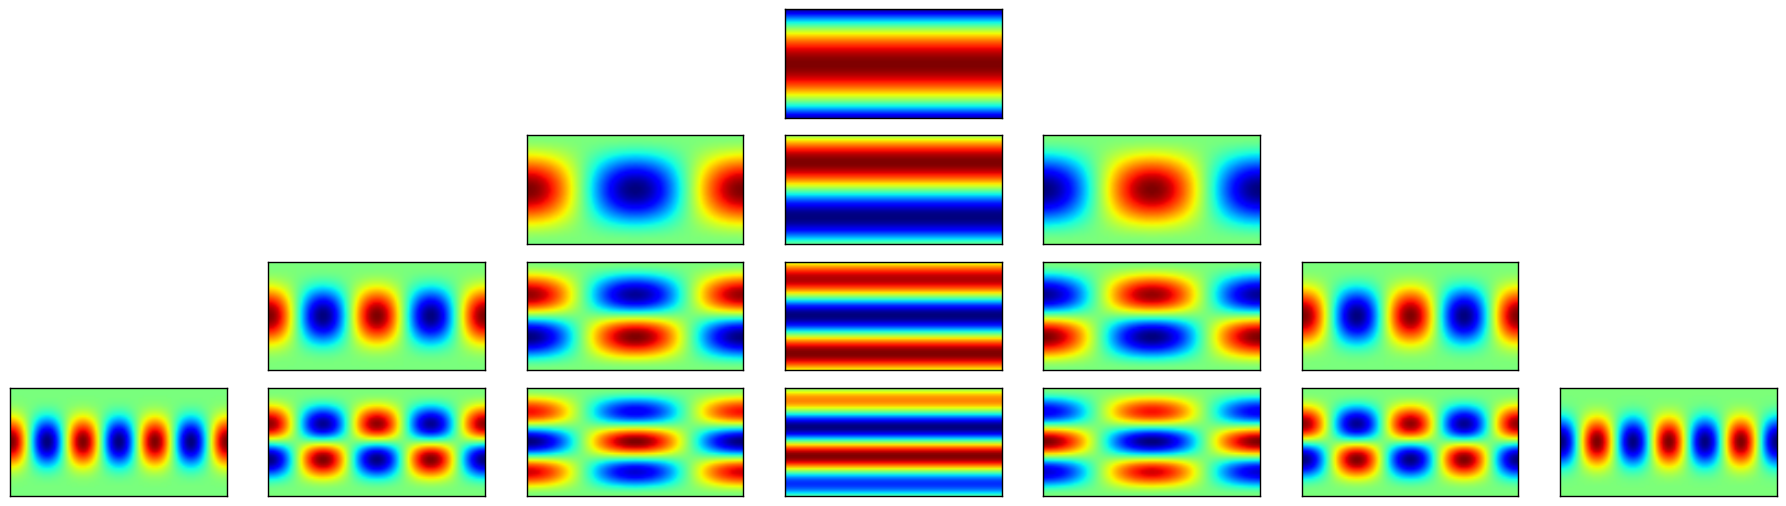
\includegraphics[width=0.45\linewidth]{q8_a_pyramid_real.png} &
  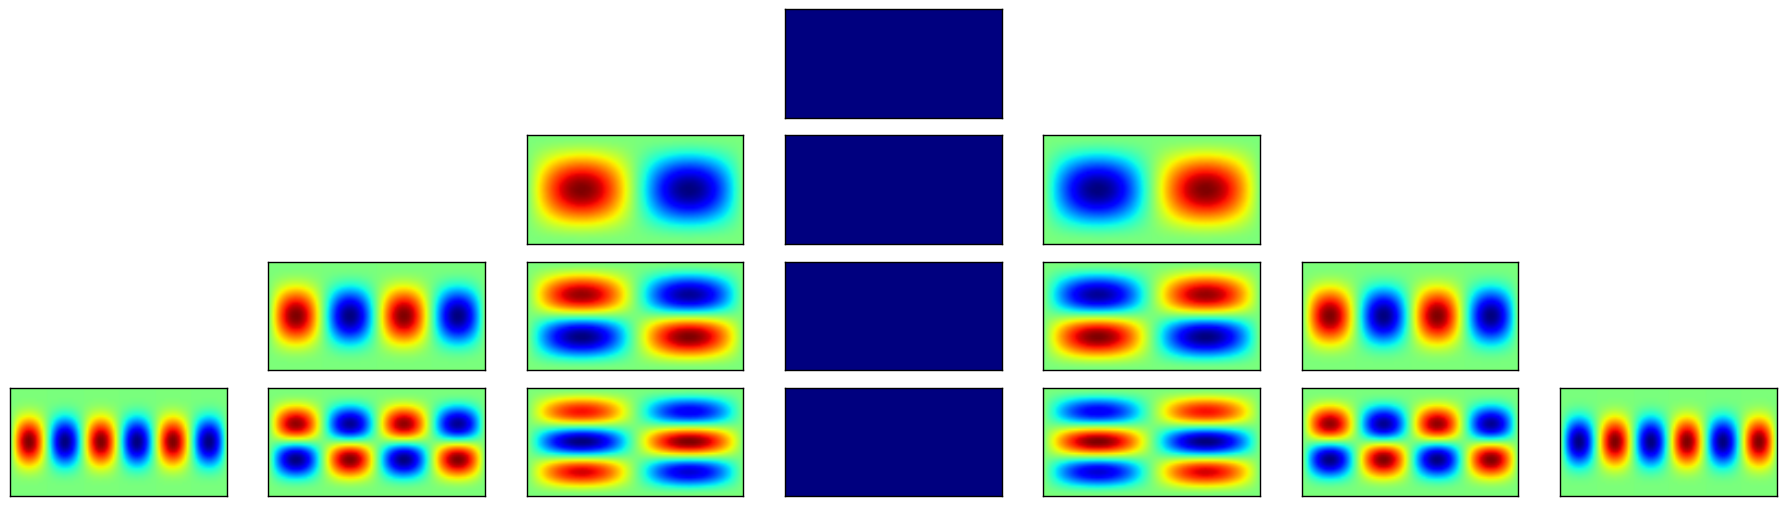
\includegraphics[width=0.45\linewidth]{q8_a_pyramid_imag.png} \\
  (a) & (b)
  \end{tabular}
  \caption[Sample Spherical Harmonics]
   {(a) Real and (b) imaginary bases of degrees 0-3 (rows) of Spherical Harmonics in latitude-longitude format, already multiplied by their solid angle. Each column is a different order, starting with 0 in the middle, 1 on its right, -1 on its left, and so on.}
   \label{q8a:sh_ex}
\end{figure}

%Just like the Fourier transform, Spherical Harmonics is a transform using a principal root of unity as its kernel. Having a kernel based on a principal root of unity over the function's domain confers a plethora of interesting attributes. One of which is that the functions generated form an orthonormal basis spanning the whole domain, called a complete orthonormal system.

%This pixelwise multiplication works because the SH basis forms an orthonormal system. Projecting something on an orthonormal basis can be called a dot product, because it yields the same properties. Thus, this relation holds \emph{iif} $f(x)$ and $g(x)$ are orthogonal over period $p$:
%\begin{equation}
%f \cdot g=\int_{-p}^p f(x)g(x)\,dx\ \quad,
%\end{equation}
%explaining why discrete transforms in general (SH, Fourier, Z, etc.) work using a single per-element multiplication.
%\todo{least squares?}

%Computing a coefficient $s$ of a given degree $n$ and order $m$ of spherical harmonic is be done by projecting the base $Y_n^m$ on the environment map $\B{L}$. Given a latitude-longitude representation,

\subsection{(b)}
\textbf{A common problem is that the signal reconstructed from SH coefficients $s$ can be negative, which is physically inconsistent when the signal represents lighting. Explain how SH coefficients $s_{\text{nonneg}}$ can be estimated from $\B{L}$, under the constraint that the reconstructed lighting be positive.}


The signal reconstructed from the Spherical Harmonic transform (using all the SH coefficients $s$ present in the signal) is proved to be exactly the same than the original signal. Negative values reconstructed from a strictly positive input cannot happen when performing the whole transform. One problem, though, is that computing the whole SH transform can be excessively long on medium to large input signals. People often take a low-frequency approximation of their signal by computing only the first SH coefficients $s$, which, when reconstructed, may bear some errors, potentially making some values becoming negative.

In such case, the one and only way to reconstruct strictly positive (or null) lighting $\bar{\B{L}}_{\mathbf{nonneg}}$ is by thresholding the reconstruction result $\bar{\B{L}}$:
\begin{equation}
\bar{\B{L}}_{\mathbf{nonneg}} = \max\left( 0, \bar{\B{L}} \right) \quad.
\end{equation}

That being said, as~\cite{Sloan2008} relate, the amount of negative lighting can be greatly reduced in two ways:
\begin{enumerate}
  \item{Performing windowing on the signal;}
  \item{Performing the projection using an optimization with regularization to enforce positive light.}
\end{enumerate}
The first involves convolving the input signal with a window such as Hanning or Lanczos to limit the ringing effect of projecting onto a base---a major cause of negative reconstruction values---, called the Gibbs phenomenon. By the convolution theorem, performing an element-wise multiplication in the frequency domain after the projection would produce an identical result in a less expensive way, in terms of computational effort. Also, windowing generally attenuates high-frequencies, making the SH reconstructed approximation even smoother than without it.

The second option changes the projection step to add a regularization, for example minimizing the curvature of the approximation:
\begin{equation}
\arg \min_s \int\left( \bar{\B{L}}(\omega) - \B{L}(\omega)\right)^2 \mathrm{d}\omega + \lambda \int \left(\Delta \bar{\B{L}}(\omega)\right)^2 \mathrm{d}\omega
\quad.
\end{equation}
While this formulation cannot be performed by a simple dot product anymore, this optimization problem can be efficiently performed using SH.

\subsection{(c)}
\textbf{As their name indicates, SH model full spherical signals. However, outdoor illumination is emitted from the sky \emph{hemisphere}. Describe Hemispherical Harmonics (HH), and how they differ from SH.}

We use the Fourier transform, Spherical Harmonics, the Z-Transform, etc. because of their useful properties, mainly the convolution theorem---element-wise multiplication in the spectral domain is a convolution in the spatial domain---, which is inherited from the orthogonality of their kernel. For example, the Fourier transform basis are all orthogonal w.r.t. each other in $\mathrm{L}^1$ space over the interval $\left[-\pi, \pi\right]$. As Spherical Harmonics are defined over a surface, its bases must be orthogonal w.r.t. each other in $\mathrm{L}^2$ space. Such set of functions were first described by Legendre as the eponymous associated polynomials $P_n^m(x)$. These associated Legendre polynomials $P_n^m(x)$ define an orthogonal basis in $\mathrm{L}^2$ over the interval $\left[ -1, 1 \right]$. To use them in spherical harmonics, this interval must be shifted to $\left[ 0, \pi \right]$ to cover the elevation of a full side of the unit sphere (from zenith to nadir). This can be done by taking the $\cos$ of the input value, giving the new bases $P_n^m\left(\cos(\theta)\right)$. Each base is multiplied by a second variable, the azimuth $\phi$ on the interval $\left[ 0, 2\pi \right[$, to get a complete sphere surface.
%For the Fourier transform, any pair of functions $\in e^{\frac{2\pi i}{N}kn}$ are orthogonal over the domain $\left[ 0, 2\pi \right]$, as $\int_{n=0}^{N}$

To define the Spherical Harmonics on hemispheres instead of whole spheres, one must shift the interval of orthogonality of the basis from $\left[ 0, \pi \right]$ (from zenith to nadir) to $\left[ 0, \frac{\pi}{2} \right]$ (from zenith to equator). Just as the Spherical Harmonics use the $\cos$ of the input values, it is possible to define the function $2\cos(\theta)-1$, which keeps the orthogonality of the original associated Legendre polynomials over the interval $\left[ 0, \frac{\pi}{2} \right]$. All the rest is the same as the Spherical Harmonics transform, aside from the normalization which should be done over half an hemisphere (over $2\pi$) instead of a full sphere (over $4\pi$).

Many different definitions are available for Hemispherical Harmonics (HH). The particular definition I just presented is available in \cite{Gautron2004}. Other definitions use different orthogonal polynomials at their core, such as the Jacobi~\cite{Makhotkin1996} or the Zernike~\cite{Koenderink1996} polynomials. While having the same properties (e.g.\ compatible with the convolution and shift theorem), each have its own advantages and disadvantages. The definition based on the Legendre polynomials is probably the most easily comparable to standard Spherical Harmonics, though. In fact, they are similar in most points: the same basis polynomial, as well as efficient rotation and evaluation. They are, however, not orthogonal to one another, so multiplying some SH coefficients with some HH coefficients won't perform a surface integral.

The main use of Hemispherical Harmonics is to represent BRDFs, though using it for sky hemisphere is a quite interesting idea. This model would, however, systematically suppose that zero energy comes from the nadir hemisphere. This could be corrected by approximating the ground BRDF (supposing we're outside) by another hemispherical harmonics transform, lighting it efficiently using the sky hemispherical harmonics and then lighting a surface element with both sky and ground combined (both using their hemispherical harmonics).

Another interesting difference between SH and HH is that, contrarily to spherical harmonics, there exist a simple formulation for hemispherical harmonics reconstruction that ensures non-negative results, as described by~\cite{Elhabian2011}.

\subsection{(d)}
\textbf{In general, the convolution $f * g$ of two spherical signals $f$ and $g$ cannot be represented on the sphere, but rather in the rotation group SO(3). However, if f or g have a specific property, then the result of $f * g$ can in fact be represented on the sphere. What is this property? How can the result of the convolution be efficiently computed using SH? Give an example of where this can be used in a practical application. \emph{Hint: think about the rendering equation.}}

As related by~\cite{Sloan2008,jarosz-08}, the convolution $f*g$ of two spherical signals $f$ an $g$ can be represented on the sphere if the basis functions are circularly symmetric (symmetric on the sphere azimuth). This means that, by the convolution theorem, a convolution in the spectral domain is the weighted multiplication of the coefficients. Each new coefficient can be computed by performing
\begin{equation}
\left(f * g\right)_n^m = \sqrt{\frac{4\pi}{2n+1}} h_n^0 f_n^m
\quad,
\end{equation}
for each degree $n$ and order $m$. This equation provides an efficient computation of the convolution, as it represents a normalized dot product in the frequency domain.

This property can be used for rendering materials efficiently, as demonstrated by~\cite{Ramamoorthi2001a}. Suppose you have an environment map $\B{L}$ on which you computed the spherical harmonics transform $\hat{\B{L}}$ and a bidirectional reflectance distribution function $\hat{f}$, also in the spherical harmonics space. To compute the irradiance $\B{E}$ of this whole surface, it is possible to perform the convolution---a dot product in the frequency domain---between the environment map and the reflectance function as follows:
\begin{align}
\B{E} &= \underbrace{\begin{minipage}{42pt}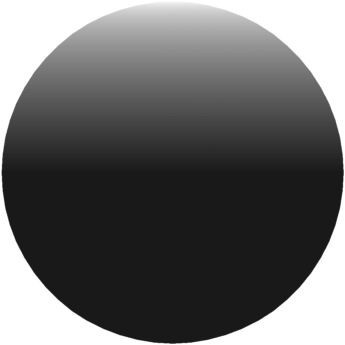
\includegraphics[width=42pt]{q8_foreshortening_sphere.png}\end{minipage}}_{f}
*
\underbrace{\begin{minipage}{42pt}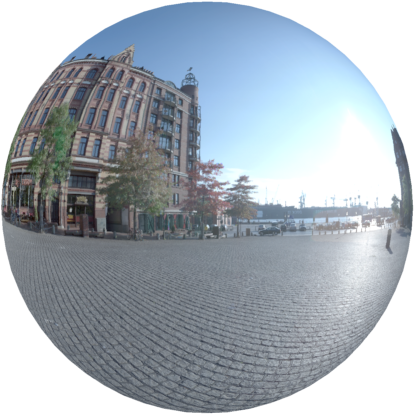
\includegraphics[width=42pt]{q8_envmap_sphere.png}\end{minipage}}_{\B{L}} \\
\hat{\B{E}} &= \sum_{n,m} \sqrt{\frac{4\pi}{2n + 1}} \hat{f}_n^m \cdot \hat{\B{L}}_n^m
\qquad,
\end{align}
for all the computed degrees $n$ and orders $m$. Performing this convolution gives the reflectance aspect of a given material for all the possible surface normals when lit by a given environment map. Rendering this object is a matter of sampling the spherical harmonic at the right normal angle (i.e.\ position on the sphere or bases), giving directly the pixel intensity. Its accuracy is limited by the number of degrees $n$ used in the transform.

% This is about rotation, not convolution: This implies that spherical harmonics basis functions are rotationally invariant, meaning that we can, for example, rotate any function in the spectral domain without aliasing by only looking at its unrotated counterpart.



\section{Question 9}

\textbf{Explain why spherical harmonics may not be well-suited for modeling high-frequency signals such as the sun. Describe an alternative representation that could better represent sunlight.}

One problem of the full spherical harmonics transform (i.e.\ all the degrees $n$ possibly present in a discrete signal) is its prohibitive computing time. As such, people generally compute only the low frequency coefficients, leading to an approximation which can be incredibly precise in some cases (e.g.\ irradiance on lambertian reflectance), but not so good in some other cases (e.g.\ outdoor radiance map). As this tuned-down version of the transform only represents low frequency components in the signal, this approximation cannot represent faithfully abrupt changes and spatially small but important variations, such as the radiance of the sun. It would need a combination of high degree coefficients to approximate it correctly, which requires substantially more computational effort than estimating the low-frequency SH coefficients, which defeats the purpose of using spherical harmonics to perform efficient convolution.

I see two alternative ways to model high-frequency signals such as the sky or the sunlight: 1) parametric (often physics-based) models and 2) non-parametric data-driven models. Many parametric sky models were developed---such as~\cite{preetham-siggraph-99,perez-se-93}---to capture the detail of the sun, the weather and the atmosphere. There is yet to come a database with enough data to describe the sky using a data-driven approach, but my feeling is that it should appear soon in the literature.

An interesting avenue to investigate would be the possibility to fit a low-frequency spherical harmonic to an environment map, superimposed with a fast-decay function (parametric or data-driven). This combination could be used to represent the sun (with the fast-decay function) and the atmosphere (with spherical harmonics).


{\small
\bibliographystyle{acm}
\bibliography{library}
}

\end{document}
